\documentclass[a4paper, openany, 12pt]{article}

%% подключаем стандарт библиографии
\bibliographystyle{gost71u}

%% для "Abstract" в классе book
% \newenvironment{abstract}{}{}
% \usepackage{abstract}

%% подключаем преамбулу: в ней содержится подключение всех необходимых пакетов
%% Работа с русским языком
\usepackage{cmap}			 % поиск в PDF
\usepackage{mathtext} 		 % русские буквы в формулах
\usepackage[T2A]{fontenc}	 % кодировка
\usepackage[utf8]{inputenc}	 % кодировка исходного текста
\usepackage[russian]{babel}	 % локализация и переносы

%% Пакеты для работы с математикой
\usepackage{amsmath,amsfonts,amssymb,amsthm,mathtools}
\usepackage{icomma}

%% Нумерация формул (опционально)
%\mathtoolsset{showonlyrefs=true} % показывать номера только у тех формул, на которые есть \eqref{} в тексте.
%\usepackage{leqno}               % нумерация формул слева

%% Шрифты
\usepackage{euscript}	 % шрифт "Евклид"
\usepackage{mathrsfs}    % красивый мат. шрифт

%% Некоторые полезные макросы для дебага (в случае недоверия авторам шаблона)
\makeatletter
\newcommand\thefontsize{The current font size is: \f@size pt} % пример: \section{\thefontsize}
\makeatother

%% Настройка размеров шрифтов
\makeatletter
\renewcommand\Huge{\@setfontsize\Huge{14pt}{1.5}}
\renewcommand\huge{\@setfontsize\huge{14pt}{1.5}}
\renewcommand\Large{\@setfontsize\Large{14pt}{1.5}}
\renewcommand\large{\@setfontsize\large{12pt}{1.5}}
\makeatother

%% Поля (геометрия страницы)
\usepackage[left=3cm,right=1.5cm,top=2cm,bottom=2cm,bindingoffset=0cm]{geometry}

%% Русские списки
\usepackage{enumitem}
\makeatletter
\AddEnumerateCounter{\asbuk}{\russian@alph}{щ}
\makeatother

%% Работа с картинками
\usepackage{caption}
\captionsetup{justification=centering} % центрирование подписей к картинкам
\usepackage{graphicx}                  % вставки рисунков
\graphicspath{{images/}{images2/}}     % папки с картинками
\setlength\fboxsep{3pt}                % отступ рамки \fbox{} от рисунка
\setlength\fboxrule{1pt}               % толщина линий рамки \fbox{}
\usepackage{wrapfig}                   % обтекание рисунков и таблиц текстом

%% Работа с таблицами
\usepackage{array,tabularx,tabulary,booktabs} % дополнительная работа с таблицами
\usepackage{longtable}                        % длинные таблицы
\usepackage{multirow}                         % слияние строк в таблице

%% Красная строка
\setlength{\parindent}{12.5mm}

%% Интервалы
\linespread{1.5}
\usepackage{multirow}

%% TikZ
\usepackage{tikz}
\usetikzlibrary{graphs,graphs.standard}

%% Верхний колонтитул
\usepackage{fancyhdr}
\pagestyle{fancy}

%% Перенос знаков в формулах (по Львовскому)
\newcommand*{\hm}[1]{#1\nobreak\discretionary{}{\hbox{$\mathsurround=0pt #1$}}{}}

%% Дополнительно
\usepackage{float}   % добавляет возможность работы с командой [H] которая улучшает расположение на странице
\usepackage{gensymb} % красивые градусы
\usepackage{caption} % пакет для подписей к рисункам, в частности, для работы caption*
\usepackage{listings} % пакет для листингов с кодом
\lstset{              % настройки для лисингов с кодом
basicstyle=\small\ttfamily,
columns=flexible,
breaklines=true
}

% Hyperref (для ссылок внутри  pdf)
\usepackage[unicode, pdftex]{hyperref}

% Отступ перед первым абзацем в каждом разделе
\usepackage{indentfirst}

\usepackage{color}
\definecolor{lightgray}{rgb}{.9,.9,.9}
\definecolor{darkgray}{rgb}{.4,.4,.4}
\definecolor{purple}{rgb}{0.65, 0.12, 0.82}
\lstdefinelanguage{JavaScript}{
  keywords={break, case, catch, continue, debugger, default, delete, do, else, false, finally, for, function, if, in, instanceof, new, null, return, switch, this, throw, true, try, typeof, var, void, while, with},
  morecomment=[l]{//},
  morecomment=[s]{/*}{*/},
  morestring=[b]',
  morestring=[b]",
  ndkeywords={class, export, boolean, throw, implements, import, this},
  keywordstyle=\color{blue}\bfseries,
  ndkeywordstyle=\color{darkgray}\bfseries,
  identifierstyle=\color{black},
  commentstyle=\color{purple}\ttfamily,
  stringstyle=\color{red}\ttfamily,
  sensitive=true
}

\lstset{
   language=JavaScript,
   backgroundcolor=\color{lightgray},
   extendedchars=true,
   basicstyle=\footnotesize\ttfamily,
   showstringspaces=false,
   showspaces=false,
   numbers=left,
   numberstyle=\footnotesize,
   numbersep=9pt,
   tabsize=2,
   breaklines=true,
   showtabs=false,
   captionpos=b
}

\begin{document}
    %% титульник
    \begin{center}
    %% *название института*
    \large\textbf{Министерство образования и науки Российской Федерации \\
    Московский физико-технический институт (государственный
    университет)} \\
    \vspace{1cm}

    %% *факультет/физтех-школа*
    Физтех-школа радиотехники и компьютерных технологий \\

    %% *название базовой кафедры и лаборатории*
    %% в случае ненадобности можно удалить
    Кафедра микропроцессорных технологий в интеллектуальных системах управления \\

    \vspace{3em}

    Выпускная квалификационная работа магистра
\end{center}

\begin{center}
    \vspace{\fill}
    %% *название вашей работы*
    \LARGE{Разработка средств инструментации бинарного файла многоязыковой виртуальной машины.}

    \vspace{\fill}
\end{center}


\begin{flushright}
    \textbf{Автор:} \\
    Студент М01-206б группы \\
    Назаров Константин Олегович \\
    \vspace{2em}
    \textbf{Научный руководитель:} \\
    Добров Андрей Дмитриевич  \\
    \vspace{2em}
    \textbf{Научный консультант:} \\
    Солдатов Антон Анатольевич \\
\end{flushright}

\vspace{7em}

\begin{center}
    %% *лого*
    \includegraphics[width=100 pt]{MIPT_logo.jpg}\\
    Москва \the\year{}
\end{center}

%% выключаем отображение номера для этой страницы (титульник)
\thispagestyle{empty}

\newpage
\setcounter{page}{2}
\fancyfoot[c]{\thepage}
%% *надпись над верхним колонтинулом*
%% в случае ненадобности можно удалить
\fancyhead[L]{Разработка средств инструментации бинарного файла многоязыковой виртуальной машины.}
\fancyhead[R]{}
    %% аннотоция
    \begin{abstract}

    \begin{center}
        \large{Разработка средств инструментации бинарного файла многоязыковой виртуальной машины.} \\
    \large\textit{Назаров Константин Олегович} \\[1 cm]

    Инструментация байткода является распространенной техникой для изменения поведения или аттрибутов программы. Эта техника может использоваться в целях профилировки, мониторинга, а также для динамического изменения поведения программы даже после сборки приложения. Существующие библиотеки для бинарной инструментации кода рассчитаны на инструментацию бинарных файлов для какого-либо языка программирования. В ходе данной работе был разработан фреймворк для работы с бинарными файлами многоязыковой платформы. Было проведено сравнение с существующими аналогами, а также показаны возможности инструментации кода, полученного из исходных файлов на разных языках.

    \vfill

    \end{center}

\end{abstract}
\newpage

    %% содержание
    \tableofcontents{}
    \newpage

    \fontsize{14}{16}\selectfont
    \section{Введение}
\label{sec:Chapter0} \index{Chapter0}

Изменение семантики программы посредством манипуляции ее бинарным кодом является распространенной техникой, используемой в современной разработке. Она используется для добавления к существующему проекту элементов рефлексии или имплементации парадигм аспекто-ориенторованного программирования (далее АОП). Зачастую, целью подобных изменений является решение существующих проблем традиционного объектно-ориентированного программирования (далее ООП). Несмотря на то, что применение ООП позволяет увеличить продуктивность разработки за счет переиспользования существующих компонент посредством таких механизмов как полиморфизм и наследование, соблюдение этих принципов не всегда возможно. Например в проектах, в которых невозможно реализовать централизованную стратегию разработки и развития всех компонент, таких как внешние библиотеки. Конечный пользователь не имеет контроля над совместимостью компонент из разных библиотек, а также не всегда имеет доступ к исходному коду, что приводит к проблеме обеспечения функциональной совместимости (интероперабельности) между компонентами. Для решения этой проблемы ООП предлагает написание классов-оберток, которые бы обеспечивали интерфейсную совместимость. Данный подход приводит к проблемам поддержки кодовой базы, а также обеспечения выполнения контрактов между компонентами. Бинарная манипуляция является альтернативным решением проблем интероперабельности. Вместо того, чтобы создавать новые классы-обертки, пользователь может модифицировать оригинальные определения в библиотеке \cite{bca}. Изменения происходят на стороне пользователя после поставки компоненты, и не требуют доступа к исходному коду.

Помимо обеспечения интероперабельности между компонентами, бинарная манипуляция также применяется для обеспечения принципа разделения обязанностей, являющегося важной частью АОП. Соблюдение этого принципа заключается в отделении разработки функциональной части приложения от имплементации нефункциональных контрактов, таких как обеспечение безопасности, поддержка единой модели распространения приложения и дргуих. Для достижения этой цели недостаточно простого изменения интерфейсов или иерархии классов, и необходимо иметь инструменты для модификации тел уже существующих функций \cite{tanter2002}.

Помимо упомянутых выше, существует еще множество областей применения бинарной инструментации. Ниже приведен более подробный разбор уже существующих задач, а также рассмотрены некоторые другие области применения данной техники.

\subsection{Интероперабельность}

Интероперабельность - это способность двух или более компонент программного обеспечения работать вместе несмотря на различия в языке, интерфейсе или исполняющей платформе \cite{malone2014}. В рамках данной работы остановимся на рассмотрении кросс-интерфейсной интероперабельности и того, как задача бинарной манипуляции связана с ней.

Существует два основных механинзма для реализации интероперабельности: стандартизация интерфейсов (Interface Standartization) и интерфейсный мост (Interface Bridging). Первый подход заключается в создании единого интерфейса и последующего приведения интерфейсов участников взаимодействия к нему. Второй подход состоит в создании взаимооднозначного соответствия между интерфейсами всех участников взаимодействия \cite{wegner1996}. Стандартизация интерфейсов зачастую явялется предпочтительным решением, поскольку является наиболее масштабируемым. Действиетльно, для данного подхода нужно построить всего $n + m$ соответствий, где $n$ - число интерфейсов первого участинка, и $m$ - число интерфейсов второго участника взаимодействия. Для второго подхода число соответствий будет равно $m * n$. Недостатком же стандартизации интерфейсов является то, что она значительно усложняет дальнейшее расширение интерфейсов, а также поддержку новых функциональностей, остутствующих в языке на момент стандартизации интерфейсов. Промышленным примером системы интероперабельности с стандартизованным интерфейсом является стандарт \texttt{Component~Object~Model~COM/OLE} компании \texttt{Microsoft}. Данный стандарт решает проблему межпроцессного взаимодействия путем предоставления единого бинарного интерфейса для представления объектов в системе \cite{brockschmidt1995}. Альтернативным подходом к решению проблемы кросс-интерфейсной интероперабельности явялется предоставление механизма для изменения интерфейсов при их загрузке в систему.

В рамках платформы \texttt{JVM} для языка \texttt{Java} данный подход был реализован в фреймворке \texttt{BCA} \cite{bca}. Данный фреймворк работает следующим образом: он предоставляет пользователю интерфейс для написания собственного трансформатора (\texttt{Modifier}), который принимает считанный бинарный файл \texttt{Java} (далее класс-файл, class-file), проводит над ним указанные пользователем манипуляции, после чего возвращает измененный файл и передает его верификатору \texttt{JVM}. При помощи бинарной манипуляции достигается интерфейсная совместимость по месту использования, что гарантирует сохранение совместимости используемых компонент, а также позволяет отложить манипуляции до непосредственно загрузки бинарного файла на платформу, что приводит к уменьшению дополнительной нагрузки на виртуальную машину.

Более подробно фреймворк \texttt{BCA} будет рассмотрен в \autoref{sec:Chapter2}.

\subsection{АОП}

Выше упоминалось, что ООП не всегда способно обеспечить выполнение принципа разделения обязанностей. Можно без труда заметить, что применение объектно-ориентированного подхода приводит к тому, что некоторые участки кода повторяются во многих классах, поскольку функциональность, реализуемая данным кодом, присуща им всем. Особенно это заметно, когда речь заходит об имплементации контрактов или не функциональных свойств системы, таких как модель обработки ошибок, проверка пост- и предусловий или аутентификация и проверка прав доступа. Для решения этих проблем была предложена парадигма АОП \cite{kiczales1997}. Основной идеей АОП стала мысль, что программист должен иметь возможность раздельно судить о функциональных и не функциональных свойствах системы.

С точки зрения АОП функиональное требование - это некоторое требование, позволяющее реализовать какую-либо концепцию, возможность или вид функциональности. Аспект же - это код, реализующий заданное функциональное требование, который запускается другими функциональными требованиями в различных ситуациях \cite{zhemzhicky}. Если функциональное требование не было выделено в аспект, то функциональность этого требования будет вызываться явно в коде, реализующем другой вид требования, что приводит к спутыванию (\texttt{cross-cutting}) этих требований. Кроме того, необходимость вызовов кода функционального требования в различных местах, приводит к рассеиванию реализации требования по многим несвязным участкам системы. В рамках АОП такая функциональность называется сквозная функциональность. Таким образом, АОП является парадигмой программирования, основанной на идее отделения сквозной функциональности от основной для улучшения разбиения программы на модули. АОП ставит своей целью разработать механизм модуляризации сквозной функциональности в объектно-ориентированных системах, предоставляя языковые средства для отделения функциональности от аспектов. Действительно, наличие модели программирования, которая предполагает реализацию таких требований единожды и их использование только в одном месте программы позволяет значительно сократить время разработки, а также улучшить читаемость и отлаживаемость кода.

В парадигме АОП каждое приложение можно поделить на классы и аспекты. Модульность в приложении достигается следующим способом: основная функциональность реализуется в виде классов, в то время как сквозная - аспектами.

Следствием того, что классическое ООП плохо справляется с проблемой отделения аспектов является широкое использование в промышленности фреймворков по типу \texttt{BREX} \cite{brex}. Данный фреймворк изолирует сегменты кода относящиеся к бизнесс-логике проекта, что помогает эффективнее менять и адаптировать правила, которым должен следовать продукт. Для достижения этой цели \texttt{BREX} производит анализ проекта в три этапа: классификация переменных (Variable Classification), идентификация бизнесс-логик (Business Rule Identification) и отображение бизнесс-логик (Business Rule Representation).

Работу данного фреймворка можно проиллюстрировать на слеюующем примере. Пусть имеется приложение, описывающее поведение людей и животных. В данном приложении имплементированы две основные функциональности. Одна является бизнесс-логикой проекта и описывает, как взаимодействия между хищниками и жертвами влияет на общую популяцию. Вторая используется для хранения статистик всех акторов участвующих в симуляции. Ниже на \autoref{fig:brexSchema} приведена схема приложения, из которой можно понять устройство проекта.

\begin{figure}[h]
\centering
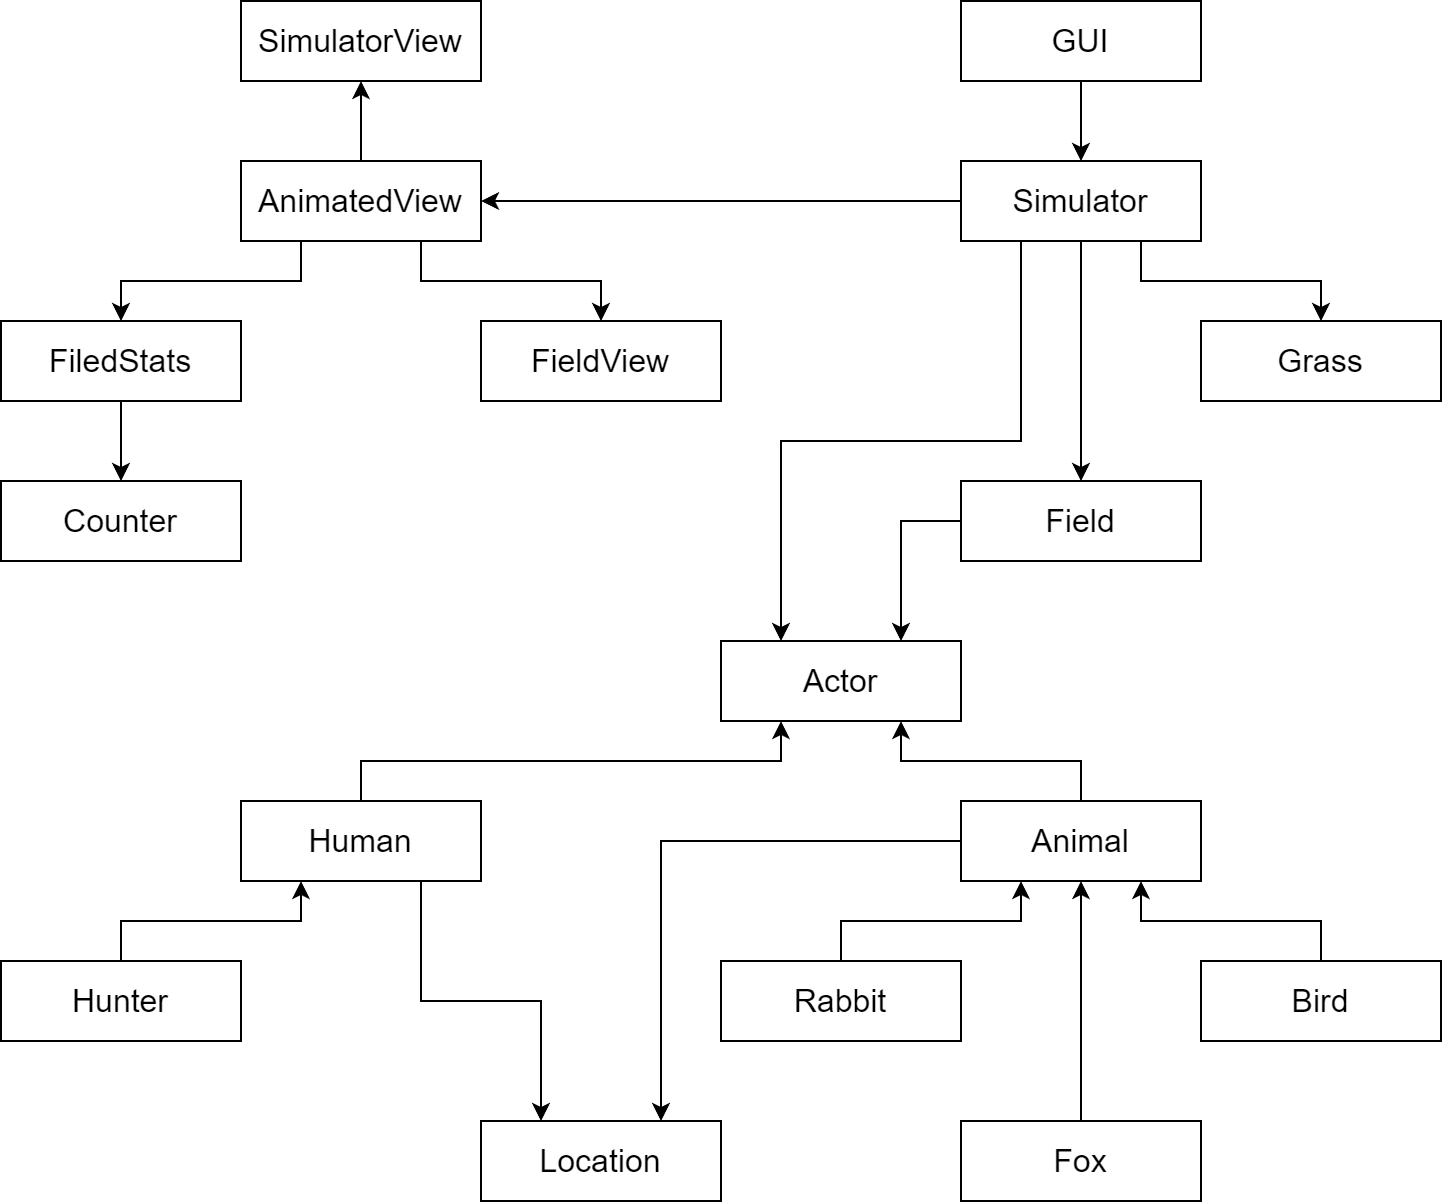
\includegraphics[width=.65\textwidth]{brex.png}
\caption{Схема зависимостей приложения.}
\label{fig:brexSchema}
\end{figure}

После применения каждой из описанных выше стадий, фреймворк выделит поетнциальные участки, относящиеся к сквозным функциональностям, присутствующим в программе. В качестве результата фреймворк генерирует диаграмму найденных связей, пример которой приведен ниже.

\begin{figure}[h]
\centering
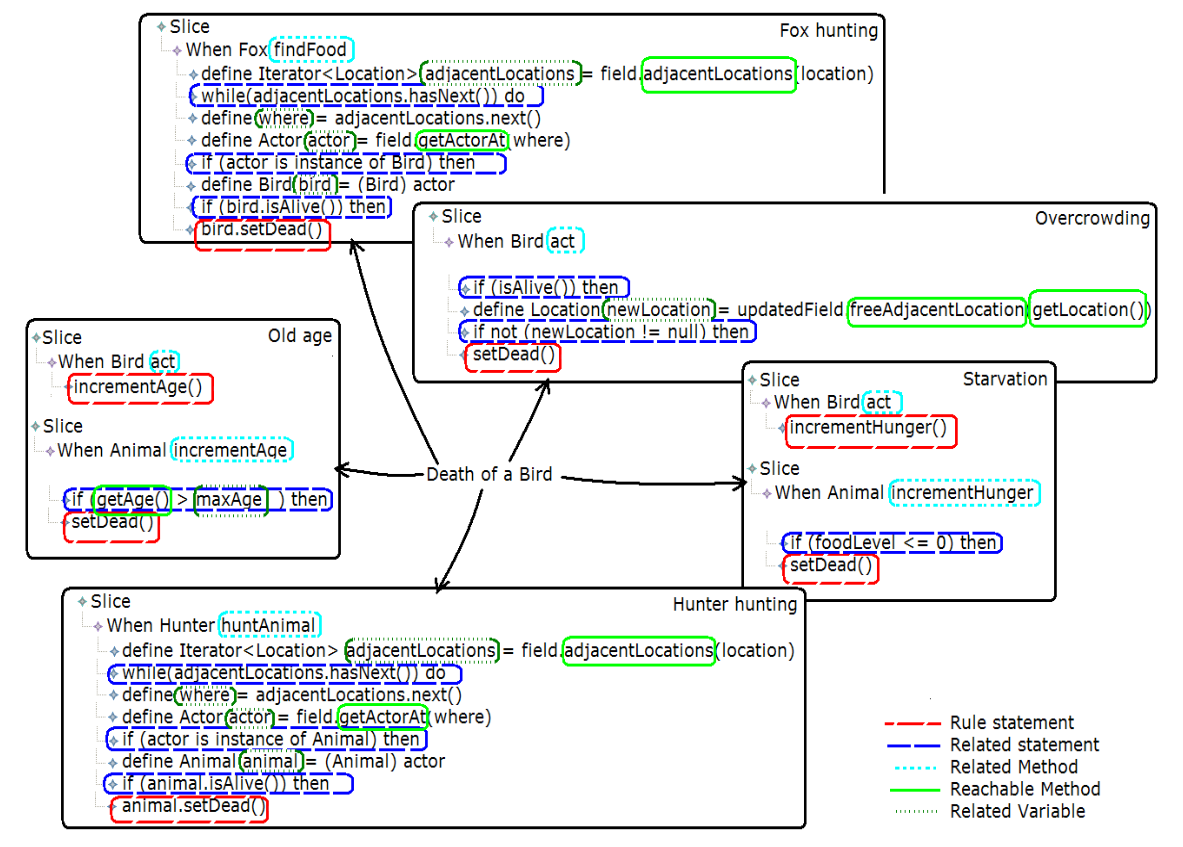
\includegraphics[width=.8\textwidth]{brex-result.png}
\caption{Результат работы фреймворка - потенциальные причины смерти птицы.}
\label{fig:brexResult}
\end{figure}

Схема на \autoref{fig:brexResult} является текстовым представлением всех условий, которые приводят к смерти птиц в данной модели. На изображении выделены различные сгенерированные бизнесс-логики, контролирующие смерть птиц, которые были обнаружены фреймворком. Данный анализ может помочь установить все явные и неявные контракты приложения, однако он не решает изначальной проблемы: кодовая база все еще не модуляризована и имеет множество сквозных функциональностей. Ниже речь пойдет о том, как внедрение элементов АОП позволяет повысить модульность проекта и избежать спутывания кода.

Поскольку широкое распространение парадигма АОП получила в языке \texttt{Java}, для него были написаны многие фреймворки, привносящие элементы АОП в язык и платформу \texttt{JVM}. Популярность АОП на платформе \texttt{JVM} объясняется в том числе относительной открытостью элементов процесса сборки к расширению. Например пользователь имеет возможность встроить свои элементы логики на многих важных этапах компиляции, таких как загрузка считанного файла в виртуальную машину или построение дерева абстрактного синтаксиса. Еще одной причиной распространенности парадигмы АОП среди \texttt{Java} приложений является наличие в языке механизма аннотаций, позволяющего помечать пользовательскими данными место определения класса, функции или поля, а также место использования типа. Данные аннотации будут сохранены в бинарный класс-файл и позже могут быть считаны как компилятором, так и во время исполнения кода рантаймом виртуальной машины посредством языковых средств рефлексии. Наличие механихма аннотаций делает естественным внедрение логик, основанных на аннотировании языковых сущностей. Более того, в самом языке \texttt{Java} определены несколько встроенных аннотаций, которые также можно считать зачатками аспекто-ориентированности в языке. Например аннотация $@Deprecated$ означает, что сущность, помеченная этой аннотацией больше не является поддерживаемой, и ее использование должно быть ограничено. Встречая использование сущности, помеченной этой аннотацией, компилятор будет генерировать соответствующее предупреждение, что будет приводить к падению процесса сборки при должных настройках \cite{javaAnnotations}.

\begin{lstlisting}[language=Java, caption=Пример использования аннотации \texttt{Deprecated}, label=lst:javaDeprecated]
/**
 * @deprecated
 * explanation of why it was deprecated
 */
@Deprecated
static void deprecatedMethod() { }
\end{lstlisting}

Выше в \autoref{lst:javaDeprecated} приведен пример использования аннотации \texttt{Deprecated}. Любое дальнейшее использование метода \texttt{deprecatedMethod} будет сопровождаться предупреждением от компилятора.

Примером того, как бинарная манипуляция может помочь с достижением модуляризации аспектов может служить следующий пользовательский сценарий, полученный из промышленной кодовой базы. Чтобы обеспечить выполнение требований к безопасности, при сборке приложения под определенное окружение разработчик может захотеть убедиться, что перед любым применением некоторого набора функций будет вызываться служебная процедура, проверяющая все необходимые для обеспечения безопасности условия. Исходя из описанного выше, наивная имплементация подобнойлогики приведет к пересечению аспекта, отвечающего за обеспечение безопасности, с основной функциональностью приложения. Чтобы избежать этого и обеспечить модульность контракта безопасности используется следующая АОП архитектура, основанная на применении пользовательских аннотаций бинарной манипуляции.

\begin{lstlisting}[language=Java, caption=Пример решения задачи замены функции в месте вызова при помощи АОП, label=lst:callSiteAOP]
// Declaration of the annotation that will be used to specify
// safe wrappers for the library API.
@interface CallSiteReplacement {
   String targetClass();
   String methodName();
}

// Class that is responsible for providing safe wrappers for the library API.
public class ApiControl {
    // Presence of this annotation means that we need to replace all calls to
    // the method `foo` from the class `com.xxx.Api` with the calls to
    // `ApiControl.WrapApiFoo`
    @CallSiteReplacement(targetClass="com.xxx.Api", methodName="foo");
    public static void wrapApiFoo(target: com.xxx.Api, ...) {
        // Logic that ensures safe use of the `foo` API.
    }
};
\end{lstlisting}

Рассмотрим \autoref{lst:callSiteAOP}. В нем приведен пример того, как может быть реализована АОП архитектура, обеспечивающая вызов безопасной обертки для библиотечного метода \texttt{foo} класса \texttt{com.xxx.Api}. Класс \texttt{ApiControl} реализует функционал, проверяющий все необходимые параметры для безопасного вызова конкретных функций библиотеки. Каждый метод этого класса - это безопасная обертка одной из библиотечных функций. Аспектом в даной архитектуре является механизм замены мета вызова на безопасный при определенных параметрах сборки. Данный аспект, как и каждый, состоит из двух частей - точки соединения (join point) и совета (advice). Точка соединения - это точка в выполняемой программе, где следует применить совет. В данном случае точкой соединения будет являться каждая конкретная инстанциация аннотации \texttt{CallSiteReplacement}. В ней указаны два параметра: \texttt{targetClass} и \texttt{methodName}. Они определяют то, вызовы какого метода должен быть заменены на безопасную обертку. Советом же в данной схеме будет являться логика преобразования бинарного файла, находящая все функции, аннотированные аннотацией \texttt{CallSiteReplacement}, и заменяющая все вызовы методов, указанных в аргументах аннотации на вызов аннотированной функции. Ниже в  \autoref{lst:callSiteAOP2} приведен пример того, как выглядит код до и после применения описанных выше трансформаций.

\begin{lstlisting}[language=Java, caption=Демонстрация работы аспекта, label=lst:callSiteAOP2]
// Before AOP.
public class MyClass {
    public static void main() {
        com.xxx.Api api = GetApi();
        api.foo(...);
    }
};

// After AOP.
public class MyClass {
    public static void main() {
        com.xxx.Api api = GetApi();
        ApiControl.wrapApiFoo(api, ...);
    }
};
\end{lstlisting}

В результате применения данной схемы реализации удается достигнуть модуляризации логики замены вызова функции на ее обертку, что избавляет кодовую базу от сквозных функциональностей, тем самым улучшая качество кода и стоимость его поддержки.

\subsection{Рефлексия}

Рефлексия - это способность системы или программы инспектировать и модифицировать собственную структуру во время исполнения. Для языка \texttt{Java} это означает изменение поведения загруженных классов, интерфейсов, методов и полей во время исполнения. Данная возможность позволяет программному обеспечению динамически изменять собственное поведение в зависимости от параметров времени исполнения. Применение рефлексии в производстве облегчает разработку и дальнейшую поддержку программ, предоставляя средства для гибкой интеграции со сторонними кодовыми базами и для отделения логики конфигурирования поведения программы в зависимости от параметров окружения в во время исполнения.

\begin{figure}[h]
\centering
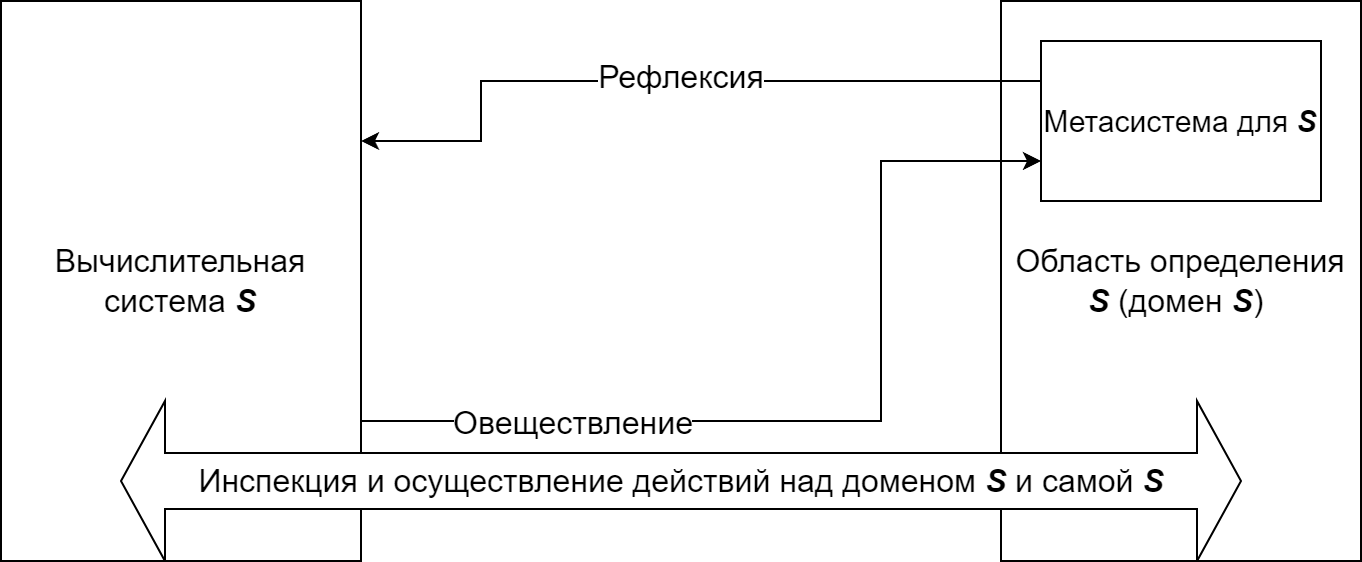
\includegraphics[width=.7\textwidth]{reflect.png}
\caption{Рефлексивная вычислительная система.}
\label{fig:reflectionScheme}
\end{figure}

Как показано на \autoref{fig:reflectionScheme}, в своем наиболее общем виде рефлексивная система может быть определена как система, удовлетворяющая следующим требованиям. Во-первых, система \texttt{S} должна иметь в своем домене собственное представление, называемое метасистемой. Это представление должно быть доступно для инспекции и манипуляции. Во-вторых, существует связь между системой \texttt{S} и ее представлением. Любое изменение в системе должно приводить к соотвествтуеющему изменению в метасистеме, и наоборот \cite{javaReflection}. Тоесть система \texttt{S} должна быть овеществлена (reified) в свое представление прежде чем метасистема может начать оперировать. Затем метасистема инспектирует и манипулирует системой средствами рефлексии используя представление \texttt{S}. Данные связи отражены подписанными стрелками на \autoref{fig:reflectionScheme}.

Несмотря на потенциальные плюсы полноценной рефлексии, многие решения, приедоставляемые стандартными библиотеками весьма ограничивают пользоваетля в возможности изменения объектов или же вовсе запрещают модификацию. Подобное решение связано с тем, что неконтролируемое испольование возможносетй рефлексии может привести к коду, о поведении которого очень сложно судить, что только ухудшает качество разработки. Однако существуют сценарии, в которых подобный подход наоборот приводит более прозрачной логике проекта. Примером такого сценария может служить задача отслеживания изменения состояния. Для достижения этой цели наиболее естественным решением будет является переопределение операции доступа к состоянию в рантайме, нежели чем написание отдельной программы, проходящейся по всем методам бинарного класс-файла и инструментирующей все операции доступа к состоянию. Помочь с имплементацией этого подхода может бинарная манипуляция. Существует множество фреймворков, использующих бинарную манипуляцию для имплементации расширений к языку. Примером подобного фреймворка может служить \texttt{Kava}, подробнее о которой будет рассказано в \autoref{sec:Chapter2}.

\subsection{Конфигурация и оптимизация}

Бинарная манипуляция также широко применяется для имплементации пользовательских оптимизаций и конфигиурации параметров кода в зависимости от параметров сборки. Как правило, такие пользовательские настройки делаются при помощи препроцессора, который способен менять структуру приложения на уровне исходного кода. Однако многие высокоуровневые языки не обладают доступным пользователю препроцессором. В качестве альтернативного решения зачастую используются фреймворки бинарной манипуляции, позволяющие изменить результирующий бинарный код аналогично тому, как препроцессор меняет исходный. Примером подобной пользовательской настройки может служить \autoref{lst:debug}

\begin{lstlisting}[language=Java, caption=Пример использования класса с конфигурацией проекта, label=lst:debug]
// Configuration class
public class Configuration {
    public static Boolean debug = False;
}

// User written code
public static class MyClass {
    public static void foo() {
        if (Configuration.debug) {
            ...
        }
        ...
    }
}
\end{lstlisting}

Для того, чтобы убрать из поставляемого пользователю бинарного файла все следы кода, используемого для отладки, авторы библиотек пишут свои собственные расширения к компилятору, использующие бинарную манипуляцию. Целью данного преобразования является удаления \texttt{true} ветки всех подобных условных операторов.

\begin{lstlisting}[language=Java, caption=Результат работы преобразования, label=lst:debug]
// After binary manipulations
public static class MyClass {
    public static void foo() {
        // `true` branch eliminated
        ...
    }
}
\end{lstlisting}

Данный подход является очень дешевым и распространенным способом настройки поведения приложения, хоть и не дает всех плюсов, обеспечиваемых парадигмой АОП.

\subsection{Актуальность}

Выше была показана востребованность инструментов бинарной манипуляции. Действительно, многие бизнесс-логики больших и даже средних компаний построены на применении описанных техник, особенно в таких языках как \texttt{Java} и \texttt{Kotlin}, где подобные инструменты имеют долгую историю развития. Поэтому, чтобы оставаться конкурентноспособной, любая платформа, намеревающаяся выйти на рынок разработки мобильных приложений, обязана предоставить свои средства для решения проблем интероперабельности компонент, поддержки принципов АОП и анализа программ посредством рефлексии или инспекции бинарных файлов. Более того, решение должно быть разработано с учетом всех особенностей платформы и предоставлять свои преимущества по сравнению с конкурирующими. В данной работе были рассмотрены дизайн и реализация библиотеки для манипуляции бинарными файлами многоязыковой платформы. Были рассмотрены особенности проектированя, связанные с необходимостью поддержки бинарных файлов, полученных из исходных файлов на разных языках, проведено сравнение с существующими решениями на других платформах, а также показано, как разработанный инструмент способен эффективно решать задачи, встречающиеся в реальных бизнесс-логиках.

\newpage
 %% Введение
    \section{Постановка задачи}
\label{sec:Chapter1} \index{Chapter1}

Данная работа ставит своей целью предоставить возможность манипуляции бинарным файлом многоязыковой платформы. В данной работе будет рассмотен вопрос о представлении языковых сущностей в рамках библиотеки, а также о разработке интерфейса для их инспекции и изменения. Помимо этого, данная работа затронет вопрос интероперабельности между различными языками. Будет предложена архитектура обобщенного пользовательского интерфейса для инспекции и модификации зависимостей между сущностями из разных языков. Вопрос манипуляции бинарными инструкциями, а также графом инструкций будет затронут лишь поверхностно.

Имея в виду области применения техники бинарной манипуляции, а также поставленную цель, можно сформулировать следующие задачи, решаемые в данной работе:

\begin{itemize}
    \item Спроектировать и разработать библиотеку для инспекции и манипуляции бинарными файлами платформы.
    \item В рамках данной библиотеки реализовать удобный интрефейс для написания сложных анализов тел функций.
    \item Предоставить единый интерфейс для использования интероперабельности между различными языками платформы.
    \item Предоставить общий интерфейс для работы с бинарными файлами полученными из разных языков.
    \item Поддержать возможность представления одного и того же языка разными кодировками бинарного файла, чтобы единообразно работать с бинарными файлами, получанными из одного исходного файла различными фронтендами.
\end{itemize}

Исходя из дальнейших планов развития платформы, к решению задачи были выдвинуты следующие требования:

\begin{itemize}
    \item Имплементированная библиотека должна быть общего назначения, чтобы позже на ее основе имплементировать специализированные фреймворки и инструменты.
    \item Имплементированная библиотека должна иметь возможность быть обернутой в высокоуровневые обертки для различных языков, чтобы предоставить пользователям платформы удобный интерфейс для инспекции и манипуляции их бинарными файлами.
    \item Интерфейс для работы с телами функций должен скрывать от пользователя наличие служебных инструкций платформы, чтобы облегчить использование библиотеки.
    \item Интефрейс для работы с бинарным файлом должен скрывать от пользователя детали имплементации бинарного файла, чтобы уменьшить зависимость пользователя от версионирования формата файла.
\end{itemize}

Как видно из постановки задач и требований к ним, в данной работе не будут рассмотрены вопросы расширения средств языков или их стандартной библиотеки.

\newpage
 %% Постановка задачи
    \section{Обзор существующих решений}
\label{sec:Chapter2} \index{Chapter2}

\sloppy

Одним из способов модификации программы является изменение ее семантики посредством рефлексии \cite{compReflection}, однако многие языки, в том числе \texttt{Java} не предоставляют поддержки для изменения семантики программы. Например, в \texttt{Java} класс \texttt{Class} объявлен \texttt{final}, что предотвращает специализацию данного класса с целью изменения семантики языковых механизмов, как это например возможно в \texttt{SmallTalk}. Исходя из этого, необходимо либо вносить изменения на уровне виртуальной машины, принося в жертву портабельность (как например делают мета-объектные протоколы (\texttt{Meta~Object~Protocol,~MOP}), такие как \texttt{Metaxa} и \texttt{IguanaJ}), либо вносить изменения на уровне бинарного кода. Любые изменения исходного кода не рассматриваются, т.к. зачастую к нему нет доступа. Именно поэтому было сделано множество различных предложений по трансформации байткода, отличающихся по уровню абстракции сущностей, с которыми работает пользователь, по выразительной мощности и по гранулярности разрешенных преобразований.

В текущей главе будут рассмотрены существующие решения для решения задачи бинарной манипуляции, а также будет проведен анализ этих решений с точки зрения их области применения и архитектуры: какие из описанных во введении задач бинарной манипуляции они решают и каким образом интегрируются в потребительские приложения.

\subsection{java.lang.classfile}

Пакет \texttt{java.lang.classfile} является нативной библиотекой для работы с бинарными класс-файлами в языке \texttt{Java} \cite{lavaLangClassfile}. Мотивацией для разработки данного решения является необходимость периодически обновлять формат бинарного класс-файла. Поскольку до недавнего времени не существовало нативного решения для манипуляции бинарными файлами, разработчикам компонент приходилось сначала ждать обновления выбранного ими фреймворка для бинарной манипуляции прежде чем переходить на новую версия файла. С введением \texttt{java.lang.classfile} разработчики стандартной библиотеки будут иметь возможность предоставить интерфейс для работы с новым форматом файла одновременно с выходом новой версии. Это позволит сторонним разработчикам инструментов и фреймворков автоматически поддерживать новейшую версию класс-файла и не зависеть от сторонних инструментов.

Отличительными особенностями \texttt{java.lang.classfile} являются следующие архитектурные решения. Во-первых, все сущности этого пакета иммутабельны. Для обновления какой либо из сущностей требуется создать новую. Во-вторых, аналогично уже существующим фреймвокам типа \texttt{ASM} \cite{asm}, данное API имеет древовидную структуру, что позволяет разработчикам при необходимости быстрее адаптировать свой код под нативное решение платформы. Помимо этого, данный пакет производит все вычисления лениво, то есть тяжелые операции по типу чтения и парсинга производятся только для тех компонент, с которыми пользователь напрямую взаимодействует. Это позволяет улучшить производительность при загрузке больших классов, что в производстве встречается очень часто. Еще одной особенностью \texttt{java.lang.classfile} является то, что хоть данное API и работает на уровне абстракции бинарного файла, оно не дает возможности пользователю напрямую изменять поля, относящиеся к деталям имплементации виртуальной машины, такие как \texttt{Constant~Pool}, \texttt{Stack~Map} и другие, что позволяет сделать применение данного API более безопасным.

Ниже в \autoref{lst:javaLangClassfile} представлен пример использования данной библиотеки для модификации существующего класса, а именно удаление из него всех методов, начинающихся со слова \texttt{debug}.

\begin{lstlisting}[language=Java, caption=Удаление методов отладки из класса при помощи библиотеки \texttt{java.lang.classfile}, label=lst:javaLangClassfile]
    ClassModel classModel = ClassFile.of().parse(bytes);
    byte[] newBytes = ClassFile.of().build(classModel.thisClass().asSymbol(),
        classBuilder -> {
            for (ClassElement ce : classModel) {
                if (!(ce instanceof MethodModel mm
                        && mm.methodName().stringValue().startsWith("debug"))) {
                    classBuilder.with(ce);
                }
            }
        });
\end{lstlisting}

\subsection{BIT}

Архитектура фреймворка \texttt{BIT} основана на наблюдении, что для достижения большей части необходимых изменений достаточно инструментации только очень ограниченного количества ключевых локаций, таких как пролог и эпилог функции, начало и конец базового блока, а также до и после конкретной инструкции. Поэтому \texttt{BIT} предоставляет интерфейс для вызова методов в каждой из этих ключевых точек \cite{bit}. Как видно из описания, данный фреймворк работает с абстракциями бинарного файла, что дает возможность увеличить гранулярность инструментации.

\begin{figure}[h]
\centering
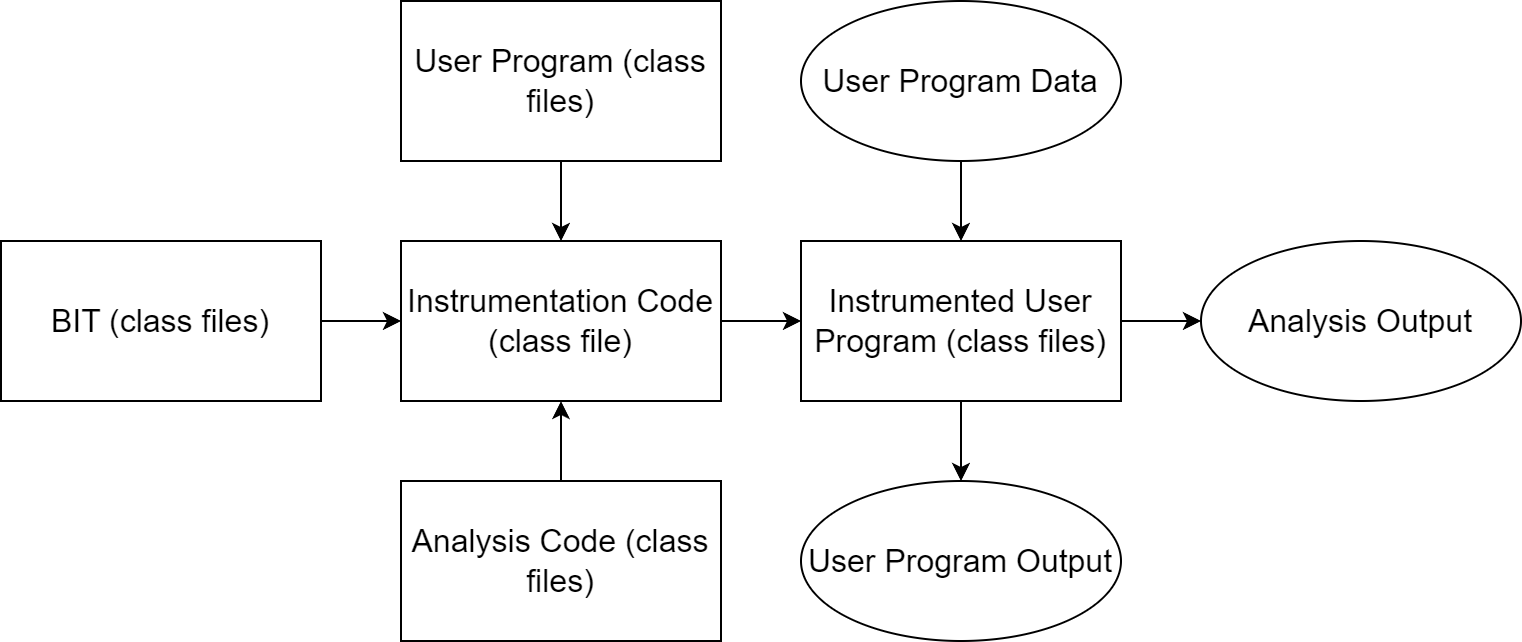
\includegraphics[width=.7\textwidth]{bit.png}
\caption{Архитектура фреймворка \texttt{BIT}.}
\label{fig:bitArch}
\end{figure}

На \autoref{fig:bitArch} проиллюстрирован процесс использования фреймворка \texttt{BIT}. Сначала пользователь пишет приложение, которое в последствии захочет инструментировать. Затем он пишет непосредственно код для инструментации и код для анализа бинарных файлов, используя классы и методы, предоставляемые фреймворком. Когда пользователь запустит код для инструментации, виртуальной машиной будут считаны бинарные файлы пользовательского приложения, после чего в нужные места пользовательского приложения будут вставлены вызовы кода для анализа. В результате получится инструментированное приложение, которое может впоследствии быть исполнено виртуальной машиной \texttt{Java}. Исполнение инструментированного приложения порождает как вывод оригинальной пользовательской программы, так и вывод анализа. Вставленные вызовы к функциям анализа ни коим образом не влияют на семантику приложения, и его вывод должен остаться неизменным.

Таким образом, \texttt{BIT} - это инструмент для создания специализированных инструментов для наблюдения и анализа поведения программ во время исполнения. \texttt{BIT} позволяет пользователям добавлять производить анализ в любом месте бинарного кода, а также получать динамическую информацию о программе во время исполнения. Подобные возможности делают \texttt{BIT} хорошим вариантом для имплементации профилировщиков и других схожих инструментов.

Ниже приведен пример того, как выглядит инструментация на фреймворке \texttt{BIT}. В \autoref{lst:Instrumentation} и \autoref{lst:Analysis} показано, каким образом будет выглядеть код для подсчета условных переходов во время исполнения.

\begin{lstlisting}[language=Java, caption=Подсчет условных переходов на \texttt{BIT}. Код инструментации, label=lst:Instrumentation]
    /* filenameIn = ...; filenameOut = ...; */
    ClassInfo ci = new ClassInfo(filenameIn);
    for (Enumeration e=ci.getRoutines().elements();e.hasMoreElements(); ){
        Routine routine = (Routine) e.nextElement();
        Vector instructions = routine.getInstructions();
        for (Enumeration b = routine.getBasicBlocks().elements(); b.hasMoreElements(); ) {
            BasicBlock bb = (BasicBlock) b.nextElement();
            Instruction instr = (Instruction)instructions.elementAt(bb.getEndAddress());
            short instr_type = InstructionTable.InstructionTypeTable[instr.getOpcode()];
            if (instr_type == InstructionTable.CONDITIONAL_INSTRUCTION) {
                instr.addBefore("BranchPrediction", "Offset", new Integer(instr.getOrigOffset()));
                instr.addBefore("BranchPrediction", "Branch", new String("BranchOutcome"));
            }
        }
        String method = new String(routine.getMethod());
        routine.addBefore("BranchPrediction", "EnterMethod", method);
        routine.addAfter("BranchPrediction", "LeaveMethod", method);
    }
    ci.write(filenameOut);
\end{lstlisting}

Заметим, что методы \texttt{addBefore} и \texttt{addAfter} добавляют вызовы к функциям, объявлены пользователем в коде анализа \autoref{lst:Analysis}.

\begin{lstlisting}[language=Java, caption=Подсчет условных переходов на \texttt{BIT}. Код анализа, label=lst:Analysis]
    public BranchPrediction {
        static Hashtable branch = null;
        static int pc = 0;
        public static void EnterMethod(String s) {
            branch = new Hashtable();
        }
        public static void LeaveMethod(String s) {
            System.out.println("stat for method: " + s);
            for (Enumeration e = branch.keys(); e.hasMoreElements(); ) {
                /* Log results */
            }
        }
        public static void Offset(int offset) {
            pc = offset;
        }
        public static void Branch(int brOutcome) {
            Branch b = (Branch) branch.get(pc);
            if (b == null)
                b = new Branch();
            if (brOutcome == 0)
                b.taken++;
            else
                b.not_taken++;
        }
    }
\end{lstlisting}

\subsection{BCA}

Фреймворк \texttt{BCA} помогает упростить составление связей между объектами путем смещения многих важных решений (например таких как имена методов или подтипирование) с времени разработки на время интеграции компонент, тем самым позволяя программистам адаптировать и применять даже сторонние библиотеки. 

\begin{figure}[h]
\centering
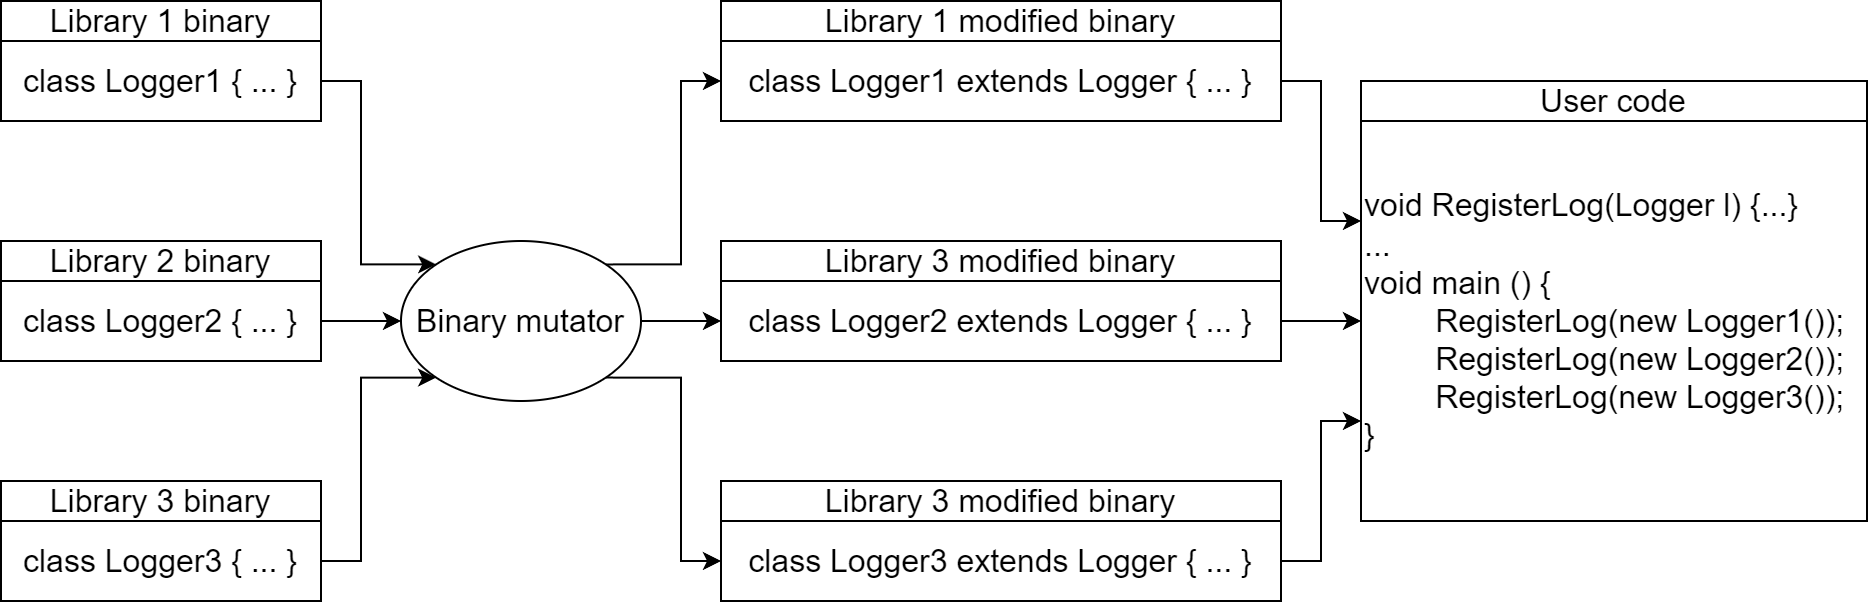
\includegraphics[width=.8\textwidth]{interoperability_example.png}
\caption{Пример использования фреймворка \texttt{BCA} для достижения интероперабельности сторонних компонент.}
\label{fig:interopExample}
\end{figure}

\texttt{BCA} изменяет компоненты во время их загрузки в виртуальную машину. Адаптация компонент происходит уже после того, как они были получены программистом, и их внутренняя структура модифицируется напрямую по месту использования. Вместо того, чтобы писать классы-обертки, происходит непосредственная модификация оригинального класса. Путем изменений бинарных файлов \texttt{BCA} удается достигнуть гибкости изменения исходного кода без сопутствующих этому недостатков:

\begin{itemize}
    \item Нет необходимости доступа к исходным файлам, что позволяет использовать фреймфорк даже на сторонних библиотеках
    \item Модификация может быть отложена до времени загрузки, что позволяет применять их по месту использования.
    \item В сравнении с модификацией исходного файла приводит к меньшему приросту времени загрузки.
    \item Модификация бинарного файла очень гибкая, и позволяет легко производить многие операции, такие как добавление нового метода, переименовывание, изменение подтипирования и иерархии классов.
\end{itemize}

Общая структура фреймворка \texttt{BCA} и его интеграция в виртуальную машину \texttt{Java} проиллюстрированы на \autoref{fig:bcaArch}.

\begin{figure}[h]
\centering
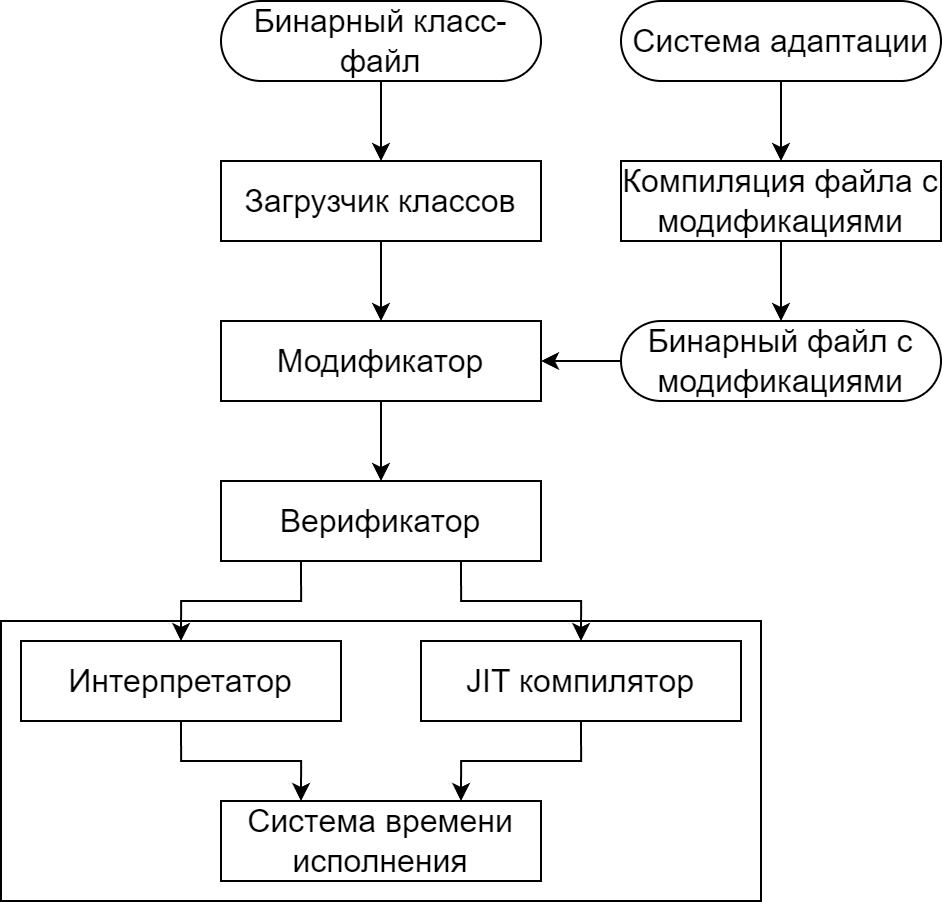
\includegraphics[width=.55\textwidth]{bca.png}
\caption{Архитектура фреймворка \texttt{BCA}.}
\label{fig:bcaArch}
\end{figure}

Когда загрузчик класс-файлов считывает бинарный файл, он строит внутреннее представление для этого файла. Во время обычного исполнения виртуальной машины \texttt{Java} это внутреннее представление сразу передается верификатору. \texttt{BCA} встраивает между этими двумя этапами, перенаправляя промежуточное представление модификатору, применяющему все необходимые трансформации к класс файлу. Все трансформации описаны в файле с модификациями (\texttt{Delta~File}), который считывается модификатором при запуске виртуальной машины. 

После модификации изменённое представление класса передается верификатору, который проверяет код на соответствие спецификации \texttt{JVM} с целью выявления недопустимых операций. После успешной верификации промежуточное представление передается в часть \texttt{JVM}, отвечающую за время исполнения. \texttt{BCA} не требует никаких изменений ни в верификатор \texttt{JVM}, ни в часть, отвечающую за время исполнения, что делает его применение более портабельным.

Чтобы гарантировать консистентность изменений, системе адаптации нужно иметь доступ ко всем файлам, которые могут быть потенциально затронуты изменениями. В случае, если весь проект хранится локально, то может быть произведена статическая адаптация компонент, в ходе которой \texttt{BCA} может просто считать все файлы и заранее применить к ним необходимые изменения, получив при этом цельное измененное приложение. Статическая адаптация имеет недостаток в том, что ей требуется дополнительное место на хранение измененного приложения, что приводит к большему потреблению дискового пространства. Однако статическая адаптация полностью убирает какие либо дополнительные затраты при загрузке классов, т.к. все трансформации уже были применены. Более того, такая адаптация позволяет публиковать код без необходимости изменений среды на стороне конечного пользователя.

Альтернативой статической адаптации является динамическая адаптация. Динамическая адаптация работает по схеме, приведенной на \autoref{fig:bcaArch}, то есть производит все манипуляции во время исполнения. Такой подход приводит к дополнительным расходам во время загрузки, что приводит к увеличению общего времени исполнения. Также динамическая адаптация требует того, чтобы файлы с модификациями распространялись вместе с приложением, и конечный пользователь использовал систему с предустановленным \texttt{BCA}. С другой стороны, динамическая адаптация не требует дополнительного места на хранение модифицированной копии приложения. Более того, в данном подходе не требуется априорное знание всех методов, которые будут загружены в приложении, что позволяет поддержать более сложные сценарии с динамической загрузкой классов (например стандартный метод \texttt{Class.forName} позволяет искать класс по имени, производя динамическую загрузку, если до этого ее не было произведено. Поскольку аргумент данной функции - строка, то не всегда есть возможность статически вычислить, чему будет равно ее значение, и статической адаптации будет недостаточно \cite{bca}).

\subsection{Kava}

Примером фреймворка, расширяющего стандартные средства рефлексии языка является \texttt{Kava} \cite{kava1} \cite{kava2}. Большинство фреймворков для манипуляции байткодом предоставляют объектно-ориентированное представление для элементов бинарного класс-файла таких как методы, типы, инструкции и других. После чего пользователю предлагается написать отдельную программу, описывающую, как переписать класс файл. Главным недостатком данного подхода является то, что для того чтобы им воспользоваться, пользователь должен обладать знаниями о байткода и формате бинарного файла платформы. Альтернативным является подход, оперирующий на языковом уровне, что несколько обезопасит и облегчит использование программистом бинарного кода. Поэтому \texttt{Kava} предлагает модель на основе поведенческой рефлексии, позволяющая изменять поведение приложения без необходимости изменения имплементации всей программы.

Для представления языковых сущностей \texttt{Kava} использует метаобъекты (\texttt{Meta~Object~Protocol}). При их помощи поведение сущностей во время исполнения, например доступ к полю, вызов метода и другие, могут быть переопределены. Метаобъекты конструируются при помощи овеществления (reification) рантайм модели объектов. Например, метод овеществляется как объект класса \texttt{Method}.

\begin{figure}[h]
\centering
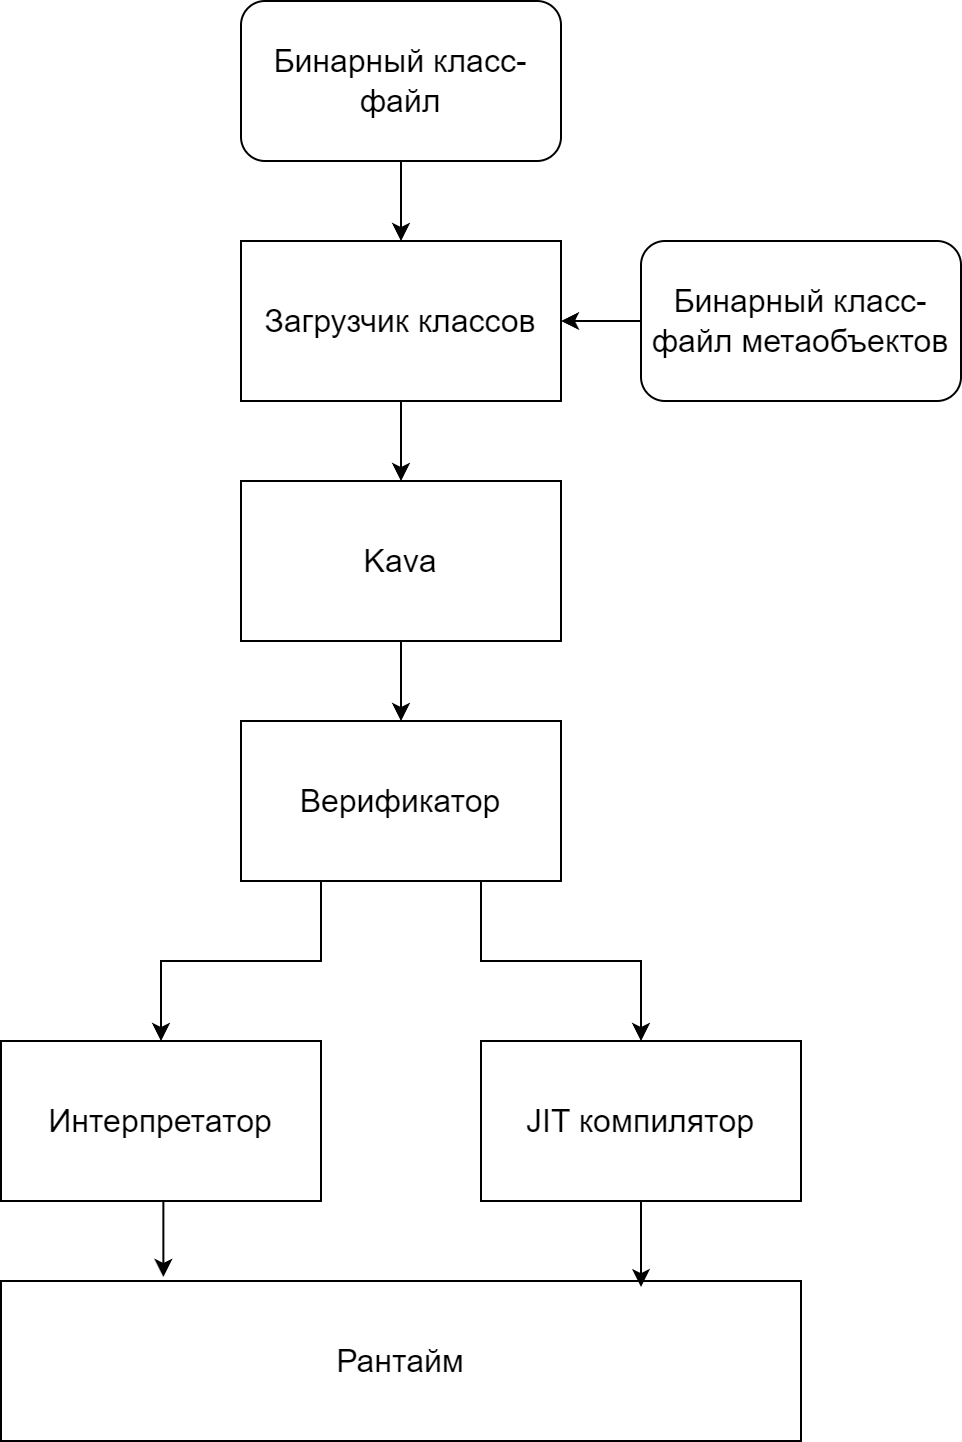
\includegraphics[width=.45\textwidth]{kava.png}
\caption{Архитектура фреймворка \texttt{Kava}.}
\label{fig:kavaArch}
\end{figure}

Как видно из \autoref{fig:kavaArch}, \texttt{Kava} реализована при помощи инструментации класс файла кодом, передающим контроль метаобъекту, ассоциированному с объектом. Для манипуляции самим байткодом \texttt{Kava} использует сторонний низкоуровневый фреймворк \texttt{BCEL}. При помощи него \texttt{Kava} инструментирует класс-файл во время его загрузки, что позволяет пользователю перехватывать и переопределять такие события как доступ к полю класса, вызов метода, вызов конструктора или выброс программой исключения.

Ниже в \autoref{lst:kava1} представлен простой пример работы с \texttt{Kava}. В нем пользователь хочет перехватить исполнение метода, поэтому он переопределяет процесс исполнения функций платформой, исполняющей \texttt{Java}. Перед исполнением функции будут выведены ее имя и дополнительная информация.

\begin{lstlisting}[language=Java, caption=Объявление метаобъекта в \texttt{Kava}, label=lst:kava1]
    public class TracingMetaObject implements MetaObject {
        public ExecutionContext beforeExecuteMethod(ExecutionContext context) {
            System.out.println("tracing " + context.getMethodName());
        }
    };
\end{lstlisting}

Для достижения желаемого результата, метаобъект должен быть привязан к классу, вызов методов которого необходимо отслеживать. Код, приведенный в \autoref{lst:kava2}, показывает как добиться отслеживания вызовов всех методов класса \texttt{Test}.

\begin{lstlisting}[language=Java, caption=Привязка класса к метаобъекту в \texttt{Kava}, label=lst:kava2]
    bind {
        class Test metaclass-is TracingMetaObject {
            any-method(any-parameters) {
                execute;
            }
        }
    }
\end{lstlisting}

Для сравнения, имплементация эквивалентной логики при помощи классического фреймворка для работы с класс-файлами приведен ниже в \autoref{lst:kava3}

\begin{lstlisting}[language=Java, caption=Реализация аналогичной функциональности при помощи классического фреймворка для работы с класс-файлом, label=lst:kava3]
    public class TraceMethod implements Constants {
        private static Method traceMethod(Method m) {
            /* Create the byte code to insert */
            /* Find insertion point */
            /* Insert byte code at beginning of method */
            /* Recalculate stack size */
            /* Return modified method */
        }
        public static void main(String[] argv) {
            /* Parse the class */
            /* Get constant pool */
            /* Generate necessary constants */
            /* Foreach method: */
            /* Call traceMethod */
            /* Write out modified class */
        }
    }
\end{lstlisting}

У данного подхода есть несколько недостатков в сравнении с реализацией через расширенный механизм рефлексии. Во первых, программист должен самостоятельно генерировать инструкции, которые необходимо вставить в бинарное представление методов, а также самостоятельно обходить класс-файл чтобы найти нужную точку вставки нового кода. Вдобавок, вставленный код может быть верифицирован только при повторной загрузке класс-файла. При помощи расширения механизма рефлексии бинарной манипуляцией, этих недостатков удается избежать.

\subsection{AspectJ}

\texttt{AspectJ} является расширением для языка \texttt{Java}, привнося в него поддержку элементов аспектно-ориентированного программирования. Данное расширение вносит в язык следующие понятия и сущности \cite{aspectj}:

\begin{itemize}
    \item Точки соединения (\texttt{Join~Points}) - однозначно определенные точки в исполнении программы.
    \item Срез (\texttt{Pointcut}) - ссылка на набор точек соединения и значения, определенные в них.
    \item Совет (\texttt{Advice}) - функционал, который определяет поведение в точке соединения.
    \item Аспект (\texttt{Aspect}) - модуль, реализующий сквозную функциональность. Аспект отвечает за применение некоего совета в точках соединения, которые определяются некоторым срезом
\end{itemize}

Далее будет приведен краткий обзор каждого из этих понятий.

Модель точки соединения является критичным элементом в любой аспектно-ориентированной системе. Данная модель предоставляет общую ``систему координат'', позволяющую координировать исполнение аспектов. \texttt{AspectJ} имплементирует модель, в которой точки соединения - это некоторые однозначно определенные точки в исполнении программы. В грубом приближении точки соединения в \texttt{AspectJ} можно представлять как узлы в графе потока управления. Получается, что поток управления проходит через каждую точку соединения дважды: первый раз на пути в поддерево, и второй раз - на обратном пути. \texttt{AspectJ} выделяет следующие виды точек соединения:

\begin{itemize}
    \item Вызов метода или конструктора - данная точка соединения находится на стороне вызывающего объекта, сразу до вызова метода или конструктора.
    \item Принятие вызова метода или конструктора - данная точка соединения находится на стороне вызываемого объекта, и находится строго до вызова метода / конструктора.
    \item Исполнение метода или конструктора - данная точка соединения находится в вызываемом методе или конструкторе
    \item Чтение или запись поля
    \item Вызов обработчика исключений
    \item Инициализация класса
    \item Инициализация объекта
\end{itemize}

Срез, как уже было сказано, это набор точек соединения с, возможно, некоторыми значениями из контекста исполнения в этих точках соединения. \texttt{AspectJ} определяет несколько примитивных срезов, которые пользователь может комбинировать, чтобы создавать свои виды срезов. Например срез \texttt{receptions(void Point.setX(int))} объединяет все точки соединения вида ``Принятие вызова метода или конструктора'', в которых сигнатура принимаемого метода равна \texttt{void Point.setX(int)}. Срезы могут комбинироваться с помощью логических операторов, как показано ниже:

\begin{lstlisting}[language=Java, caption={Срез, следящий за координатой точки \texttt{x} или \texttt{y}.}]
    receptions(void Point.setX(int)) || receptions(void Point.setY(int))
\end{lstlisting}

Пользователь также может определять собственные срезы:

\begin{lstlisting}[language=Java, caption={Пользовательский срез, следящий за координатой точки \texttt{x} или \texttt{y}.}]
    pointcut moves():
        receptions(void FigureElement.incrXY(int, int)) ||
        receptions(void Line.setP1(Point)) ||
        receptions(void Line.setP2(Point)) ||
        receptions(void Point.setX(int)) ||
        receptions(void Point.setY(int));
\end{lstlisting}

Совет - это функциональный механизм, использующийся для декларации логики, вызываемой в каждой из точек соединения в срезе. \texttt{AspectJ} определяет три вида советов - \texttt{before}, \texttt{after} и \texttt{around}. Совет определяется путем соотнесения куска кода с срезом и промежутком времени, относительно которого должен будет быть применен код в каждой из точек соединения. Например совет:

\begin{lstlisting}[language=Java, caption={Совет, отмечающий изменения точки \texttt{x} или \texttt{y}.}]
    after(): moves() {
        flag = true;
    }
\end{lstlisting}

определяет совет в срезе \texttt{moves()}. Этот совет выставляет флаг каждый раз когда исполнение выйдет из среза \texttt{moves()}.

Аспекты - это модули, определяющие сквозную логику. Декларация аспекта ведет себя как декларация класса. Внутри него могут быть определены срезу, советы и другие декларации, допустимые внутри класса. Ниже приведен пример декларации аспекта, следящего за тем, была ли фигура передвинута.

\begin{lstlisting}[language=Java, caption={Аспект, отслеживающий изменения фигур.}]
aspect MoveTracking {
    static boolean flag = false;
    static boolean testAndClear() {
        boolean result = flag;
        flag = false;
        return result;
    }
    pointcut moves():
        receptions(void FigureElement.incrXY(int, int)) ||
        receptions(void Line.setP1(Point)) ||
        receptions(void Line.setP2(Point)) ||
        receptions(void Point.setX(int)) ||
        receptions(void Point.setY(int));
    after(): moves() {
        flag = true;
    }
}
\end{lstlisting}


Советы аспекта чем-то похожи на методы в том смысле что имеют доступ к всем членам аспекта. В данном случае совет \texttt{after()} может спокойно работать со статическим полем \texttt{flag}.

Как видно из примеров, применение \texttt{AspectJ} позволяет имплементировать сквозную логику в виде отдельных модулей, тем самым явно выражая ее в одном месте. Благодаря этому, различные инструменты имеют возможность понимать сквозную логику проекта и давать программисту релевантные подсказки.

\subsection{Javassist}

Подобно \texttt{AspectJ}, \texttt{Javassist} является расширением языка \texttt{Java}, с той лишь разницей, что \texttt{Javassist} ставит своей целью расширить возможности встроенного функционала рефлексии. Данный фреймворк, как и \texttt{BCA}, может быть применен как статически, так и динамически. \texttt{Javassist} был разработать с целью упростить и обезопасить процесс инструментации финального файла и убрать необходимость рядовому разработчику проникать в детали работы виртуальной машины. Поэтому для имплементации этого фреймворка был выбран уровень абстракции исходного кода. Этот выбор приводит к уменьшению гибкости интерфейса, но с другой стороны позволяет сделать его более удобным для разработчика. Также в \texttt{Javassist} существует набор методов, позволяющих работать с байткодом напрямую. Помимо предоставления абстракций на уровне исходного кода, \texttt{Javassist} автоматически обновляет места использования модифицированных сущностей. Например, если имя класса было изменено, то оно будет изменено и в тех местах, где это имя используется.

Для работы с исходным кодом \texttt{Javassist} не использует полноценный java компилятор, поскольку полноценная компиляция \texttt{Java} кода довольно медленный процесс, и как правило, для работы функций фреймворка требуется скомпилировать только тело метода, не создавая при этом классов и другие вспомогательные структуры, которые присутствуют в бинарном класс-файле. Для обеспечения быстродействия компиляции, \texttt{Javassist} использует собственный компилятор, транслирующий только тело метода и вставляет его байткод в уже существующий метод.

Для обеспечения безопасности трансформаций, \texttt{Javassist} позволяет производить только ограниченный набор изменений. Например, в классе невозможно удалить поле или метод, можно только изменить тело уже существующего метода, или нельзя изменять сигнатуру существующего метода.

Приведем пример пользования данного фреймворка для инструментации кода. Рассмотрим пример, в котором пользователь выводит значения аргументов функции. Пусть есть метод, описанный в \autoref{lst:javassistExample}.

\begin{lstlisting}[language=Java, caption=Исходный класс, label=lst:javassistExample]
public class Point {
    int x, y;
    void move(int dx, int dy) {
        x += dx; y += dy;
    }
}
\end{lstlisting}

Для вставки логирующего кода, пользователь должен написать последовательность инструкций, описанную на \autoref{lst:javassistCode}.

\begin{lstlisting}[language=Java, caption={Код, добавляющий логирование}, label=lst:javassistCode]
    /* ... */
    ClassPool pool = ClassPool.getDefault();
    CtClass cc = pool.get("Point");
    CtMethod m = cc.getDeclaredMethod("move");
    m.insertBefore("{ System.out.println($1); System.out.println($2); }");
    cc.writeFile();
    /* ... */
\end{lstlisting}

\subsection{ASM}

Аналогично \texttt{BCA}, фреймворк \texttt{ASM} \cite{asm} поддерживает как статический режим трансформации, так и динамический, являющийся для \texttt{ASM} основным режимом работы. Поэтому как имплементация фреймворка, так и его пользовательский интерфейс заточены под то, чтобы уменьшить дополнительные расходы на работу с класс-файлами во время загрузки.

\texttt{ASM} поддерживает два варианта пользовательского интерфейса: событийный и объектно-ориентированный. Рассмотрим каждый из них по отдельности.

Событийный пользовательский интерфейс является изначальным интерфейсом \texttt{ASM} и призван решить главную проблему объектно-ориентированного представления: создание большого числа объектов для репрезентации элементов класса при загрузке, что приводит к падению производительности и увеличению расходов памяти виртуальной машины. Данный интерфейс реализован при помощи шаблона посетитель (\texttt{Visitor~Design~Pattern}). Применение данного шаблона позволяет изменять как бинарный код методов, так и структуру класса без необходимости создания объекта на каждую из сущностей, что позволяет \texttt{ASM} значительно уменьшить накладные расходы при загрузке классов.

Объектно-ориентированный интерфейс представляет класс в виде дерева объектов, в котором каждый объект осуществляет некую сущность принадлежащую классу, такую как сам класс, его поле, метод, и другие. Каждый объект содержит ссылки на объекты, осуществляющие принадлежащие ему сущности. Помимо этого, объектно-ориентированный интерфейс предоставляет функционал для преобразования древовидного представления в событийное и обратно. Другими словами, объектно-ориентированный интерфейс реализован поверх событийного интерфейса.

Каждый из этих интерфейсов имеет как свои преимущества, так и свои недостатка. Например, как было сказано выше, событийный интерфейс работает быстрее и требует меньше памяти, чем объектно-ориентированный. Однако такой интерфейс пригоден только для написания достаточно простых преобразований, поскольку в любой момент доступен только один из элементов класса, соответствующий текущему посещаемому элементу. Объектно-ориентированный интерфейс решает эту проблему, предоставляя пользователю доступ сразу ко всей модели класса, но ценой дополнительных расходов на построение дерева объектов.

Сравним эти два интерфейса на следующем примере. Пусть пользователю нужно создать код для метода в \autoref{lst:asmfoo}

\begin{lstlisting}[language=Java, caption=Необходимый метод., label=lst:asmfoo]
public class MyClass {
    int fld = 1;
    public int getFld() {
        return this.fld;
    }
}
\end{lstlisting}

Используя событийный интерфейс, создание инструкций данного метода достигается следующей последовательностью вызовов \autoref{lst:asmVisitor}.

\begin{lstlisting}[language=Java, caption=Пример использования событийного интерфейса., label=lst:asmVisitor]
    mv.visitCode();
    mv.visitVarInsn(ALOAD, 0);
    mv.visitFieldInsn(GETFIELD, "pkg/MyClass", "fld", "I");
    mv.visitInsn(IRETURN);
    mv.visitMaxs(1, 1);
    mv.visitEnd();
\end{lstlisting}

Ту же самую логику можно выразить при помощи объектно-ориентированного интерфейса \autoref{lst:asmOOP}.

\begin{lstlisting}[language=Java, caption=Пример использования объектно-ориентированного интерфейса., label=lst:asmOOP]
    MethodNode mn = new MethodNode(/* ... */);
    InsnList il = mn.instructions;
    il.add(new VarInsnNode(ILOAD, 1));
    LabelNode label = new LabelNode();
    il.add(new JumpInsnNode(IFLT, label));
    il.add(new VarInsnNode(ALOAD, 0));
    il.add(new VarInsnNode(ILOAD, 1));
    /* ... */
\end{lstlisting}

Интерфейс для работы с инструкциями автоматически осуществляет поддержку таких служебных сущностей как constant pool. Проведение анализа потока управления осуществляется при помощи отдельной функциональности \texttt{ASM}, позволяющей строить графовое представление функций. Анализ же потока данных осуществляется при абстрактной интерпретации, позволяющей смоделировать все возможные пути исполнения инструкций в методе для получения всех возможных значений ее аргументов.

\subsection{Анализ существующих решений}

Все рассмотренные в данном разделе решения можно сравнивать по множеству признаков, таких как уровень абстракции сущностей, назначение фреймворка, требуется ли глубокое знание бинарного кода для работы с ним, и другим. В ходе данной работы такое сравнение было проведено, в результате чего была получена следующая таблица:

\begin{figure}[h]
\centering
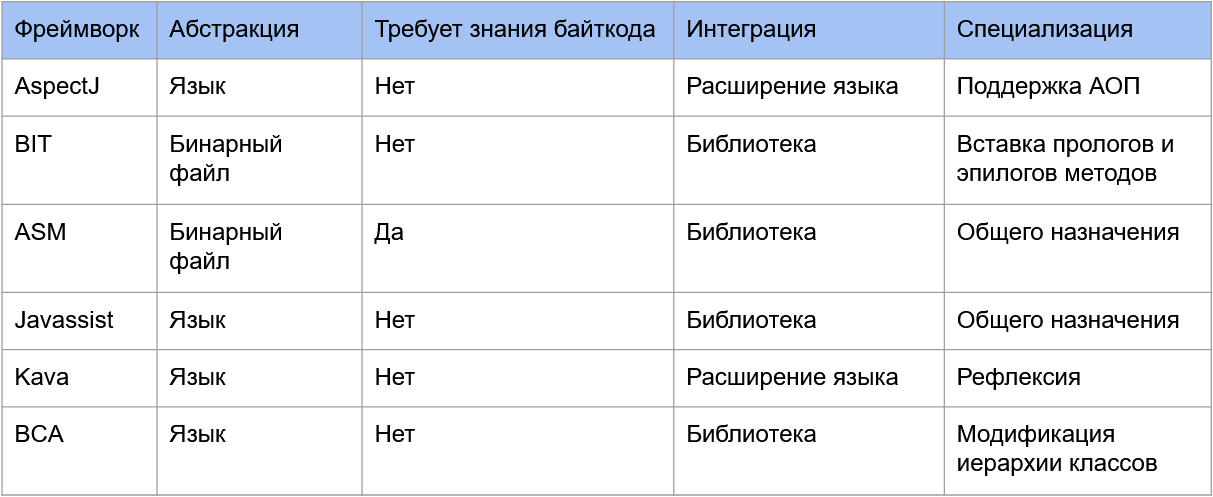
\includegraphics[width=\textwidth]{framework_comparison.png}
\caption{Сравнение рассмотренных фреймворков.}
\label{fig:kavaArch}
\end{figure}

Изучив ее и требования, выдвинутые при построении задачи, был сделан вывод, что ни одно из существующих решений не выполняет в полной мере поставленные перед данной работой задачи, из-за чего требуется более детальное рассмотрение каждого из фреймворков по отдельности и выделение из его архитектуры необходимых нам аспектов.

\newpage
 %% Обзор существующих решений
    \section{Исследование и построение решения задачи}
\label{sec:Chapter3} \index{Chapter3}

В предыдущей главе были рассмотрены различные решения для задачи бинарной манипуляции. На основе их анализа составим более детальный план решения задач, обозначенных в \autoref{sec:Chapter1}.

Задача разработки библиотеки для инспекции и манипуляции бинарными файлами разбивается на две части: разработка интерфейса для работы с бинарными инструкциями и разработка интерфейса для работы с метаданными бинарного файла. как говорилось раньше, в данной работе подробно будет рассмотрена только вторая часть интерфейса, подробное описание которго будет в \autoref{sec:Chapter4}.

Задача реализации интерфейса, удобного для написания сложных анализов тел функций сводится к выбору промежуточного представления для тел функций и написанию интерфейса, имплементирующего его. Отдельной задачей является проектировние и имплементация механизма, обеспечивающего выполнение требования скрывать от пользователя наличие служебных инструкций платформы. Данные задачи можно решать непосредственно, и подробный процесс будет описан далее в \autoref{sec:Chapter4}.

Предоставление интерфейса для использования интреоперабельности между языками платформы является самодостаточной задачей, решение которой будет представлено в \autoref{sec:Chapter4}.

Задача разработки общего интерфейса для бинарных файлов, полученных из исходных файлов написанных на разных языках, вместе с требованием поддержать возможность представления одного и того же языка разными кодировками бинарного файла, а также с требованием скрыть от пользователя детали имплементации бинарного файла говорит о том, что в разрабатываемой библиотеке должен использоваться уровень абстракции языковых сущностей. Таким образом, задача сводится к проектированию необходимых языковых абстракций и механизма овеществления различных кодировок в единое представление. Отдельной задачей является дизайн и имплементация интерфейса поверх выделенных абстракций. Для имплементации решения данной задачи был полезен анализ фреймворка \texttt{BCA}, интерфейс которого позволяет пользователю работать напрямую с языковыми понятиями, такими как наследование, избегая необходимости вникать в детали бинарного файла. Также был полезен анализ фреймворка \texttt{ASM}, который показал удобство ограниченного применения шаблона посетителя для анализа метаданных бинарного файла.

\newpage
 %% Исследование и построение решения задачи
    \section{Описание практической части}
\label{sec:Chapter4} \index{Chapter4}

После того, как все большие задачи из \autoref{sec:Chapter1} были разбиты на подзадачи, которые можно рассматривать непосредственно, перейдем к описанию их решения.

Чтобы удовлетворить требованию предоставить возможность обертки библиотеки в языки более высокого уровня, для написания публичного интерфейса был выбран язык \texttt{C}. Главным плюсом этого языка в данном случае является наличие нативных интерфейсов для него у многих современных языков программирования. Примером таких интерфейсов может служить \texttt{JNI} (\texttt{Java~Native~Interface}) \cite{jni} у языка \texttt{Java} или \texttt{N-API} (\texttt{Node~API}) \cite{napi} для языка \texttt{JavaScript}. Данные интерфейсы позволяют пользователю писать код, изменяющий параметры время исполнения. Например, \texttt{JNI} позволяет регистрировать функции, написанные на языке \texttt{C}, в качестве встроенных (\texttt{native}) функций платформы, которые в последствии можно вызывать из языка \texttt{Java}.

Поскольку для написания пользовательского интерфейса был выбран язык \texttt{C}, в котором нет возможности явно указывать приватные и публичные поля структур, то было принято решение имплементировать все сущности библиотеки как непрозрачные указатели. Эта техника позволяет разработчикам библиотеки не открывать пользователям деталей имплементации структур, вынуждая их использовать исключительно предоставленный библиотекой интерфейс. Необходимый эффект достигается путем вынесения определений структур в исходные файлы, что оставляет только декларации в заголовочных файлах. Таким образом, пользователь, подключивший себе заголовочный файл библиотеки, имеет только декларации библиотечных типов, в то время как имплементация библиотеки имеет доступ к полноценным определениям. Однако у данной техники есть один большой недостаток - отсутствие value-семантики у библиотечных типов в пользовательском интерфейсе. Действительно, поскольку пользователю недоступны определения типов, то пользовательский интерфейс может содержать только указатели на них. В рамках языка \texttt{C} это приводит к дополнительным вопросам про владение указаелем: кто аллоцировал память для объекта по указателю и чья обязанность ее освободить? В рамках данной библиотеки было решено проводить все аллокации строго на внутренних аренах библиотеки, и выдавать пользователю указатели на них. Это снимает с пользователя необходимость что-либо аллоцировать или освобождать на своей стороне для работы с интерфейсом библиотеки.

Общая архитектура библиотеки представлена на \autoref{fig:libScheme}.

\begin{figure}[h]
\centering
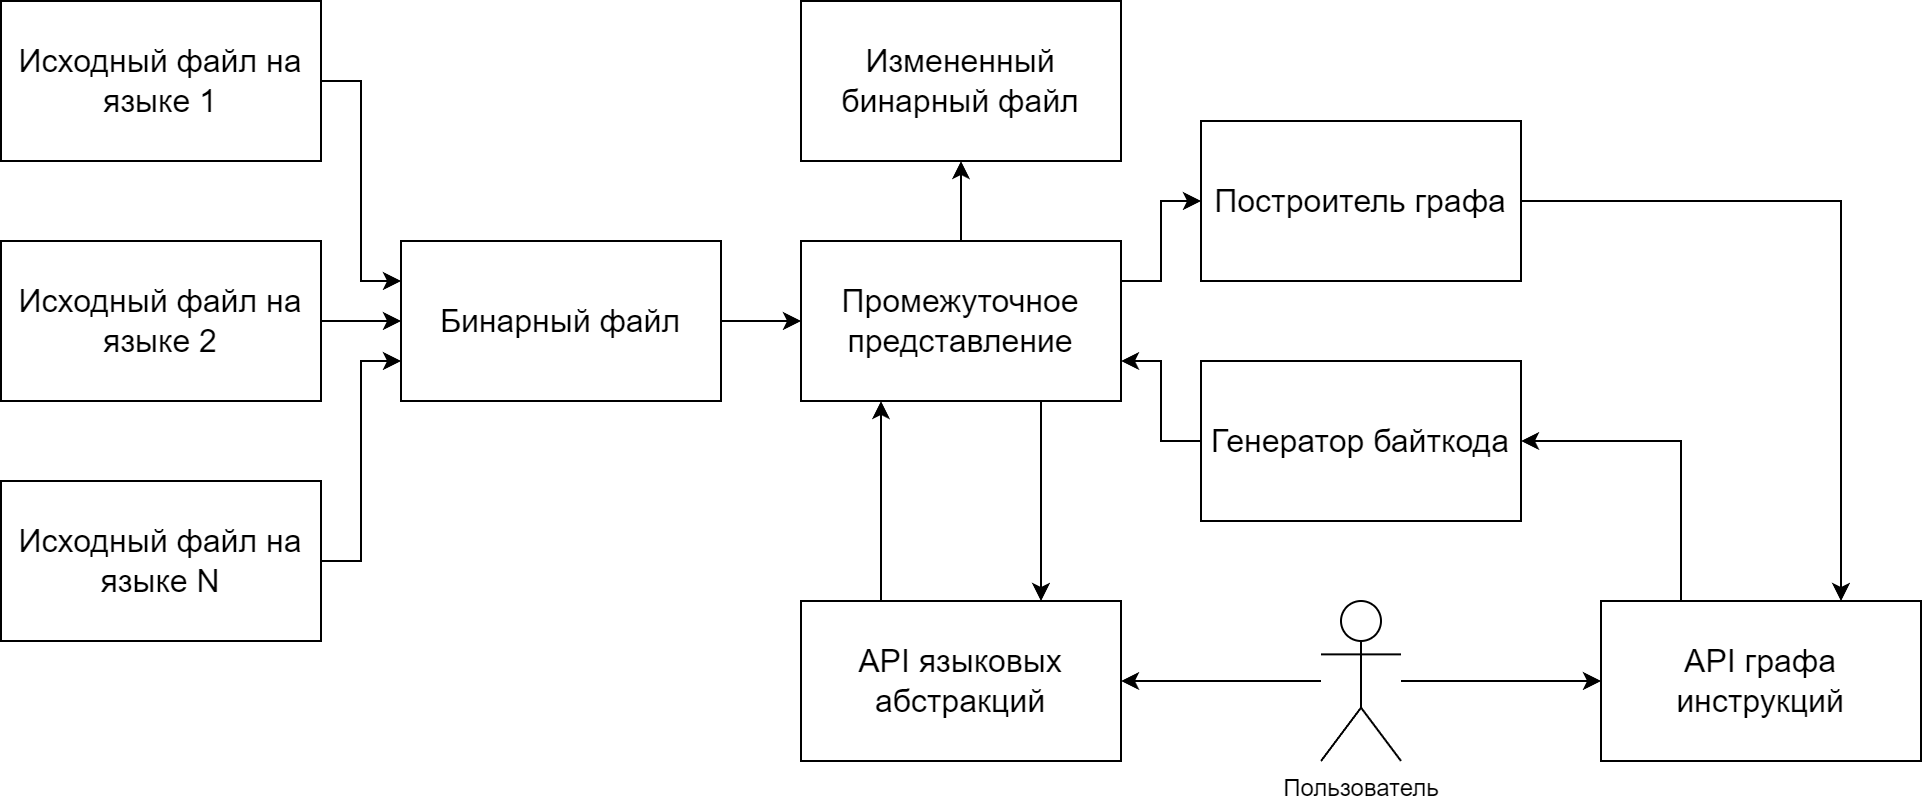
\includegraphics[width=.8\textwidth]{library_scheme.png}
\caption{Общая схема работы библиотеки.}
\label{fig:libScheme}
\end{figure}

Входной точкой пользовательского интерфейса библиотеки является бинарный файл. Он может быть получен после компиляции пользователем кода при помощи любого из возможных фронтендов платформы. Во время загрузки библиотекой бинарного файла происходит построение промежуточного представления всех структур, овеществялющих языковые абстракции, закодированные в бинарном файле. Далее, пользователь имеет возможность работать с этим представлением посредством двух интерфейсов. Первый позволяет работать с метаданными файла, такими как типы, определения функций и другие. Второй интерфейс служит для работы с телами функций, а также бинарными инструкциями.

\subsection{Фронтенд}

Для начала кратко опишем архитектуру фронтенда многоязыковой платформы, в рамках которой разрабатывается описываемая библиотека. Рассмотрим то, каким образом генерируется бинарный файл, какова его структура, и как он в дальнейшем исполняется.

Для того чтобы поддержать исполнение нескольких языков программирования в рамках одной плафтормы, необходимо решить задачу компиляции их исходных и бинарных файлов в представление, поддерживаемое платформой. С этой целью на платформе были имплементированы несколько фронтендов, каждый из которых компилирует исходный или бинарный входной файл в бинарный формат платформы. Благодаря единому бинарному формату в рамках платформы становится возможным написание таких инструментов, как описанный в данной работе, а также достигается бесшовная интероперация между различными языками.

Однако для эффективных компиляции и исполнения различных языков требуется разный по семантике набор бинарных инструкций. Это требование возникает из-за отличного поведения сущностей во время компиляции и во время исполнения. Проиллюстрируем это рассмотрением двух больших групп исполняемых на виртуальных машинах (\texttt{managed}) языков: статических и динамических. Примером статического \texttt{managed} языка могут являться \texttt{Java} или \texttt{Kotlin}. Данные языки статически типизированы, тоесть тип в них не является частью значения, поэтому например все обращения к полям объектов в них могут быть вычислены во время компиляции кода. Это позволяет компилятору и загрузчику осущесвтлять множество анализов и верифицировать код на предмет выполнения языковых гарантий, таких как связанные с модификаторами доступа сущностей. Для поддержки возможности верификации кода даже после компиляции исходных файлов требуется сохранение всей необходимой информации на уровне бинарных инструкций, что влияет на проектирование набора инструкций в виртуальных машинах, исполняющих эти языки программирования. Рассмотрим процесс обращения к полю класса в языке \texttt{Java}. Скомпилировав код, показанный в \autoref{lst:javaSource} компилятором \texttt{JVM} получим последовательность бинарных инструкций, показанную в \autoref{lst:javaBc}.

\begin{lstlisting}[language=Java, caption=Исходный код языка \texttt{Java}., label=lst:javaSource]
    public class MyClass {
        public int a = 1;
        public static int b = 2;
    };
    public class Main {
        public static void main() {
                MyClass my = new MyClass();
                int res = my.a + MyClass.b;
        }
    }
\end{lstlisting}

\begin{lstlisting}[caption=Бинарный код виртуальной машины \texttt{JVM}., label=lst:javaBc]
    public class MyClass
    public int a;
        descriptor: I
        flags: ACC_PUBLIC
    public static int b;
        descriptor: I
        flags: ACC_PUBLIC, ACC_STATIC

    public class Main
    Constant pool:
        ...
        #7 = Class #8 // MyClass
        #8 = Utf8 MyClass
        ...
        #10 = Fieldref #7.#11 // MyClass.a:I
        #11 = NameAndType #12:#13 // a:I
        #12 = Utf8 a
        #13 = Utf8 I
        #14 = Fieldref #7.#15 // MyClass.b:I
        #15 = NameAndType #16:#13 // b:I
        #16 = Utf8 b
        ...
    public static void main();
        ...
        getfield #10 // Field MyClass.a:I
        getstatic #14 // Field MyClass.b:I
        iadd
        ...
\end{lstlisting}

Как видно из листинга бинарного кода \autoref{lst:javaBc}, обращения к полям класса \texttt{MyClass} в методе \texttt{main} имеют всю необходимую типовую информацию, необходимую для проверок даже после компиляции. Действительно, поскольку аргументом инструкций доступа к полю является полный дескриптор необходимого поля, загрузчик имеет возможность найти это поле среди загружаемых классов и проверить все флаги доступа. Подобное проектирование инструкций позволяет имплементировать безопасное и надежное исполнение программ даже после применения к коду бинарных манипуляций.

Классическим примером динамического managed языка программирования является \texttt{JavaScript}. Поскольку этот язык динамический, тип в нем является частью значения переменной, и не может быть выведен фронтендом во время компиляции. Более того, из-за того, что объект в данном языке - это коллекция пар ключ-значение, из который можно как удалять, так и добавлять пары, то ни о какой верификации инструкций во время загрузки не может быть и речи. Более того, меняется семантика доступа к полю объекта, что находит свое отражение в наборе инструкций, которым оперируют виртуальные машины, исполняющие данный язык. Проиллюстрируем отличия в семантике достпа к полю объекта на примере бинарного кода виртуальной машины машины \texttt{V8}. Написав код, аналогичный \autoref{lst:javaSource}, получим следующий результат.

\begin{lstlisting}[language=Javascript, caption=Исходный код языка \texttt{JavaScript}., label=lst:jsSource]
    class MyClass {
        static a = 1;
        b = 2;
    }
    function main() {
        let my = new MyClass();
        let res = my.b + MyClass.a
    }
    main()
\end{lstlisting}

\begin{lstlisting}[caption=Бинарный код виртуальной машины \texttt{V8}., label=lst:jsBc]
    [generated bytecode for function: main (0x0e93e5d98a29 <SharedFunctionInfo main>)]
    Constant pool
        ...
        0: ... <String[7]: #MyClass>
        1: ... <String[1]: #b>
        2: ... <String[1]: #a>
        ...
    Bytecode
        ...
        ThrowReferenceErrorIfHole [0]       // #MyClass
        Star2
        Construct r2, r0-r0, [0]
        Star0
        GetNamedProperty r0, [1], [3]       // #b
        Star2
        LdaImmutableCurrentContextSlot [2]
        ThrowReferenceErrorIfHole [0]       // #MyClass
        Star3
        GetNamedProperty r3, [2], [5]       // #a
        Add r2, [2]
        ...
\end{lstlisting}

Как видно из \autoref{lst:jsBc}, в динамическом языке совершенно другая семантика обращения к полю. Во-первых, обращение к статическому и к динамическому полю выражается единой инструкцией - \texttt{GetNamedProperty}. Во-вторых, никакой информации, которая могла бы быть полезна при верификации не может быть сохранено и не сохраняется в виду модели объекта в данном языке. Также, поскольку в динамических языках тип является свойством значения, в общем случае фронтенд не может вывести, что складываются два целочисленных значения. Поэтому в отличие от \texttt{Java}, где использовалась специализированная инструкция \texttt{addi}, в \autoref{lst:jsBc} используется общая операция \texttt{Add}.

В виду этих и еще многих различий семантик исполнения различных языков, на платформе имплементировано несколько расширяемых наборов инструкций (\texttt{ISA}), каждый из которых исполняется на одной из виртуальных машин платформы в зависимости от исходного языка приложения.

Поскольку приложения могут быть написаны на нескольких языках программирования, то после линковки всех бинарных файлов приложения может оказаться так, что в рамках одного бинарного файла будет присутствовать бинарное представление сущностей из разных языков.

Это является большой проблемой для пользователей, пытающихся прочитать и проинтерпретировать бинарный файл, поскольку разные фронтенды могут по-разному кодировать необходимые ему языковые сущности в рамках одного бинарного формата. Так например фронтенду для виртуальной машины, имплементирующей спецификацию языка \texttt{JavaScript} \texttt{ECMA-262} нет смысла кодировать пользовательский класс никак иначе, кроме как функцию, в то время как фронтенду языка \texttt{Java} нет смысла кодирвать класс иначе как структуру с фиксированными разметкой и модификаторами доступа. Аналогично, фронтенду языка \texttt{JavaScript} нет необходимости сохранять информацию о типах или о сигнатурах функций, но для исполнения языка \texttt{Java} эта информация является критичной. Кроме того, некоторые фронетнды могут использовать структуры бинарных файлов для хранения имплементационных деталей, не имеющих прямого отображения на исходный код. Таким образом мы получаем ситуацию, когда каждая сущность в бинарном файле может быть интерпретирована по-разному в зависимости исходного языка и использованного фронтенда. Отсюда возникает требование скрыть такие сложные детали имплементации бинарного формата от пользователя.

Далее будут отдельно рассмотрены две части пользовательского интерфейса: интерфейс для работы с метаданными бинарного файла и интерфейс для работы с бинарными инструкциями. При рассмотрении каждого из них будет представлена его архитектура, а также то, как ее имплементация решает обговоренные выше подзадачи. Подробно в данной работе будет рассмотрен только интерфейс для работы с метаданными файла.

\subsection{Интерфейс для работы с метаданными бинарного файла}

Как уже было сказано ранее, для имплементации интерфейса для работы с метаданными бинарного файла был выбран уровень абстракции языковых сущностей. Данное решение было продиктовано желанием скрыть от пользователей платформы сложное устройство бинарного файла, а также убрать необходимость пользователю разбираться в деталях имплементации различных фронтендов платформы.

Однако данное решение требует аккуратного выбора набора языковых сущностей, с которыми будет работать библиотека, поскольку их должно быть достаточно чтобы выразить все необходимые языковые абстракции поддерживаемых языков, но при этом они должны быть достаточно общими, чтобы не создавать ситуации, когда пользователь путается, какую языковую сущность ему необходимо применить в том или ином случае.

Для выделения таких сущностей было проведено сравнение распространенных managed языков программирования. Сравнение проводилось в два этапа: сначала языки сравнивались по набору поддерживаемых языковых сущностей, затем сравнивалась их семантика: какие операции к ним применимы, а какие - нет.

В результате сравнения языков \texttt{JavaScript}, \texttt{TypeScript}, \texttt{Java}, \texttt{Kotlin} и нативного статического языка платформы был выделен следующий набор сущностей, достаточный для того, чтобы оперировать этими языками.

\begin{itemize}
    \item Класс (\texttt{Class}) - общее обозначение для всех структур данных.
    \item Функция (\texttt{Function}) - общее обозначение для всех видов функций. Анонимных функций, методов, свободных функций и дргуих.
    \item Поле (\texttt{Field}) - общее обозначение для полей чего-либо. Класса, интерфейса, пространства имен и других.
    \item Перечисление (\texttt{Enum}) - обозначение для типов перечисления.
    \item Пространство имен (\texttt{Namespace}) - обознчание для пространств имен.
    \item Аннотация (\texttt{Annotation}) и Декоратор (\texttt{Decorator}) - являются взаимоисключающими понятиями, поскольку обозначают статический и динамический механизмы добавления метаданных к декларациям.
\end{itemize}

Поскольку, как уже было обозначено ранее, один бинарный файл может содержать сущности из нескольких разных языков, в рамках библиотеки было решено адаптировать следующую модель бинарного файла. Бинарный файл - это коллекция сущностей, называемых модуль (\texttt{Module}). Модуль же - это именованная коллекция языко-специфичных деклараций, у которой есть свой публичный интерфейс, и свой список внешних зависимостей. Поскольку каждый язык имеет собственный механизм работы с внешними зависимостями, а также способ обозначения публичного интерфейса, было решено ввести абстракиции, обобщающие понятия внешней зависимости и сущности из публичного интерфейса модуля. Ими являются дескриптор импорта \texttt{Import~Descriptor} и дескриптор экспорта \texttt{Export~Descriptor}. Целью введения этих дескрипторов является отделение понятия внешней зависимости и публичного интерфейса от языко-специфичной нагрузки и предоставление некоего общего интерфейса для работы с ними, оставив при этом возможность работать с ними в контексте конкретного языка. С помощью понятий модуль, дескриптор импорта и дескриптор экспорта возможно описать общий механизм отношений между модулями и сущнстями из модулей, что позволяет библиотеке единообразно обрабатывать сценарии интероперабельности и сценарии работы с внешними зависимостями в рамках одного языка. Данный механизм является строго необходимым, поскольку различия в механизмах взаимодействия с внешними сущностями у различных языков во время компиляции и во время исполнения могут радикально отличаться. Так, например, для языка \texttt{Java} каждая импортируемая сущность может быть разрешена в класс, метод или поле класса во время компиляции проекта. После чего данные сущности могут быть сохранены в бинарном файле с пометкой \texttt{external}. Во время исполнения программы будут загружены класс-файлы с их определениями и код будет иметь возможность быть исполеннным. Из-за такой имплементации работы с внешними сущностями, на инструкций работа с внешним и локальным классом абсолютно не отличается. Однако для такого языка как \texttt{JavaScript} ни о каком разрешении имен до начала времени исполнения речи идти не может, поэтому вся информация о внешних зависимостях и публичном интерфейсе согласно спецификации \texttt{ECMA-262} хранится в отдельной для каждого модуля таблице. Данный подход очевидно отражается на наборе инструкций, с которыми работает виртуальная машина, имплементирующая данную спецификацию. Среди них появляются инструкции, работающие непосредственно с вхождениями в этой таблице. Целью введения понятий дескриптора импорта и дескриптора экспорта как раз и является сокрытие подобных деталей имплементации от пользователя и вынесение понятий внешней зависимости и публичного интерфейса модуля в языко-независимую чать библиотеки, чтобы упростить интерфейс работы с интероперабельностью.

Также, чтобы отразить факт того, что поддерживаемые платформой языки будут скомпилированы в один из ограниченного числа наборов инструкций, поддерживаемых виртуальными машинами платформы, было введено понятие \texttt{Target}, соединяющее в себе как исходный язык, так и спользуемый при его компиляции набор инструкций. Например один и тот же код на языке \texttt{Java} может быть представлен совершенно разными наборами инструкций на разных платформах, таких как \texttt{JVM} и \texttt{ART}. В рамках нашей библиотеки этот факт отразился бы в определении двух \texttt{Target}-ов для языка \texttt{Java}: \texttt{lib\_Core\_Target\_Java\_ART} и \texttt{lib\_Core\_Target\_Java\_JVM}.

Анализ семантики выделенных выше языковых сущностей показал, что функционал, применимый к данным сущностям можно разбить на две основные группы: общий и языко-специфичный.

Общий функционал над сущностями библиотеки имеет одно и то же семантическое значение для всех языков. Например взятие имени у функции или у класса. Также, в общий функционал входят те функции, для которых можно однозначно определить поведение во всех языках. В них входят функции-перечислители, принимающие функцию-посетитель в качестве аргумента (как например функция \texttt{ClassEnumerateFields} или \texttt{ClassEnumerateMethods}). Для языков, в которых данные операции имеют смысл (например \texttt{Java}), происходит вызов функции-посетителя, а для языков, в которых операции смысла не имеют (например \texttt{JavaScript}), просто ничего не происходит, и функция-посетитель не вызызвается ни разу.

Таким образом, основная часть пользовательского интерфейса состоит из следующих сущностей:

\begin{itemize}
    \item Объявления всех библиотечных типов. В эти объявления входят как служебные типы, такие как тип, строка и тп, так и обозначенные выше языковые сущности. Всем подобным типам соответствуют имена вида \texttt{lib\_Core\_XXX}, где \texttt{Core} означает принадлежность к основной части интерфейса, а \texttt{XXX} заменяется на имя сущности, описываемой типом, например \texttt{lib\_Core\_Class} или \texttt{lib\_Core\_Type}.
    \item Все функции-перечислители для объявленных типов. Поскольку поведение таких функций было однозначно определено выше для всех возможных языков, они могут стать частью общего интерфейса.
    \item Все функции-геттеры, для которых возможно определить однозначеное поведение для всех возможных языков.
    \item Интерфейс для модификации всех языко-независимых сущностей: \texttt{lib\_Core\_File}, \texttt{lib\_Core\_String}, \texttt{lib\_Core\_Type}, \texttt{lib\_Core\_Value} и других.
\end{itemize}

Задачей языко-специфичного интерфейса является определить, какие из основных сущностей релевантны для конкретного языка, а также определить функционал, применимый только к ним. Языко-специфичный интерфейс состоит из множества языковых расширений, каждое из которых определяет специфику отдельного языка. Каждое расширение определяет свой набор \texttt{lib\_<LANG>\_XXX} сущностей, специализирующих \texttt{lib\_Core\_XXX} сущности из основной части библиотеки. Каждое из расширений определяет только те сущности, которые ему нужны. Так, например, расширению \texttt{JavaScript} не нужно будет определять свой \texttt{lib\_JavaScript\_Field}, поскольку понятие поля в данном расширении не имеет смысла. Таким образом, внутренняя имплементация структуры \texttt{lib\_Core\_Class} будет выглядеть следующим образом:

\begin{lstlisting}[language=Java, caption=Внутренняя имплементация типа \texttt{lib\_Core\_Class}, label=lst:libClass]
    struct lib_Core_Class {
        /* Used to determiine correct type of `impl`. */
        lib_Core_Module* m;
        /* ... */
        union {
            lib_JS_Class* JS;
            lib_Java_Class* Java;
            /* ... */
        } impl;
    };
\end{lstlisting}

Расширения, как уже было сказано выше, определяют языко-специфичный функционал только над специализированными сущностями из основной части интерфейса. Каждое расширение имплементирует языковой инстерфейс для одного или более \texttt{Target}-ов, поскольку языковые метаданные определяются исходным языком, а не выбранным набором инструкций. Для работы с функционалом расширения пользователям необходимы функции-конверторы между сущностями основной части и сущностями расширения:

\begin{lstlisting}[language=Java, caption=Пример функций-конверторов., label=lst:libConvertors]
    struct lib_Java_Api {
        /* ... */
        CoreClassGetJavaClass,  // Converts lib_Core_Class* to lib_Java_Class*
        JavaClassGetCoreClass,  // Converts lib_Java_Class* to lib_Core_Class*
        /* ... */
    };
\end{lstlisting}

Поскольку большая часть модификаций сущностей требует языко-специфичного набора параметров, в рамках библиотеки было решено вынести весь интерфейс для модификации языковых сущностей в расширения, где модификации будут определены для канкретных специализаций \texttt{lib\_<LANG>\_XXX}.

Также, языковые расширения содержат методы для инспекции метаданных всех \texttt{lib\_<LANG>\_XXX} сущностей, поскольку большая часть метаданных является языко-специфичной, и для функций-геттеров невозможно определить общего поведения. Функции-геттеры, вынесенные в основную часть не дублируются в расширении.

Поскольку механизм работы с внешними сущностями определяется парой языков (экспортируемый-экспортирующий или импортируемый-импортирующий), каждое расширение должно предоставить собственный интерфейс для работы с импортами и экспортами. Этот интерфейс должен включать в себя добавление и удаление внешних зависимостей, а также добавление и удаление сущностей из публичного интерфейса модуля. Еще одной важной частью интерфейса является извлечение из дескрипторов языко-специфичных данных. Так, для языка Java мы можем извлечь из дескриптора импорта \texttt{lib\_Java\_Class}, \texttt{lib\_Java\_Field}, \texttt{lib\_Java\_Function}. Тем самым, каждое расширение определяет возможности своего языка к интероперабельнсти, задавая пары языков, между которыми возможно построение отношений экспорт-импорт или импорт-экспорт. Это позволяет определять правила преобразований между различными механизмами работы с внешними сущностями в частном порядке для каждой конкретной пары.

Резюмируя сказанное выше, роль языковых расширений состоит в следующем: основная часть пользовательского интерфейса для работы с метаданными предоставляет общий интерфейс, позволяющий писать общий код для работы с любым исходным языком; этот интерфейс строится поверх внутренних и публичных функций расширений. Расширения предоставляют языко-специфичный функционал, работающий только с сущностями из расширения.

Ниже представлен пример того, как может выглядеть расширение для языка \texttt{TypeScript}.

\begin{lstlisting}[language=Java, caption=Примерный код расширения \texttt{Typescript}., label=lst:libTsExtension]
    /* Declaring language-specific entities. */
    struct lib_TS_Module;
    struct lib_TS_Class;
    struct lib_TS_Function;
    struct lib_TS_Decorator;
    struct lib_TS_Namespace;
    /* etc. */

    struct lib_Api_TS
    {
        /* lib_TS_Module */
        /*
         * Note, how pair AddImport/AddExport defines,
         * which languages are supported for interop with extension's language.
         */
        ModuleAddImportFromJS(lib_TS_Module* importing, lib_JS_Module* imported, ... payload);
        ModuleAddExportFromJS(lib_TS_Module* exporting, lib_JS_Module* exported, ... payload);
        ModuleAddImportFromTS(lib_TS_Module* importing, lib_TS_Module* imported, ... payload);
        ModuleAddExportFromTS(lib_TS_Module* exporting, lib_TS_Module* exported, ... payload);
        /* etc. */
        ModuleRemoveImport(lib_TS_Module* m, lib_Core_ImportDescriptor* id);
        ModuleRemoveExport(lib_TS_Module* m, lib_Core_ExportDescriptor* ed);
        TSModuleGetCoreModule(lib_TS_Module* m),
        CoreModuleGetTSModule(lib_Core_Module* m),

        /* lib_TS_Namespace */
        TSNamespaceGetConstructorFunction(lib_TS_Namespace* ns),
        TSNamespaceGetCoreNamespace(lib_TS_Namespace* ns),
        CoreNamespaceGetTSNamespace(lib_Core_Namespace* ns),

        /* lib_TS_Enum */
        /* lib_TS_Class */
        /* lib_TS_Function */
        /* etc. */
    };
\end{lstlisting}

Комбинируя использование функций из общего интерфейса и функций из языко-специфичных расширений, пользователь может писать безопасную общкю логику, расширяемую по необходимости языко-специфичными действиями. Ниже приведен пример такого кода. Пусть перед пользователем стоит задача обойти все функции в бинарном файле. Он знает, что в языке \texttt{TypeScript} пространство имен представлено немедленно-вызываемой функцией \texttt{IIFE~(Immediately~Invoked~Function~Expression)}, которую пользователь также хочет обработать как обычную функцию. Данную логику можно выразить следующим образом:

\begin{lstlisting}[language=C, label=lst:getTsNamespace]
    static bool NamespaceEnumerator(lib_Core_Namespace* ns, void* data) {
        /* ... */

        /*
         * I, as user, know that TS namespace can contain expressions,
         * and this logic is not present in the `Core` part. So language-specific
         * behaviour is needed in order to process namespace's constructor.
         */
        lib_Core_Module* m = api_core->NamespaceGetModule(ns)
        if (lib_Core_Target_TS == api_core->ModuleGetTartget(m)) {
            auto ts_namespace = api_ts->CoreNamespaceGetTSNamespace(ns);
            auto ts_ns_ctor = api_ts->NamespaceGetConstructor(ts_namespace);
            auto ns_ctor = api_ts->TSFunctionGetCoreFunction(ts_ns_ctor);
            (void)FunctionEnumerator(ns_ctor, data);
        }

        /* ... */
    }
\end{lstlisting}


\subsection{Интерфейс для работы с бинарными инструкциями}

Как уже было сказано ранее, в рамках рассматриваемой платформы имплементировано несколько наборов инструкций, поддерживаемых различными виртуальными машинами. Все языки программирования, поддерживаемые на платформе транслируются в один из этих наборов инструкций в зависимости от используемого фронтенда. Каждый из имеющихся на платформе наборов инструкций является регистровым, с одним выделенным регистром, называемым аккумулятором, использующимся как неявный регистр для сохранения возвращаемого значения. Данный дизайн инструкций позволяет уменьшить размер инструкций за счет того, что нет необходимости кодировать регистр для возвращаемого значения, что приводит к уменьшению размера кода вцелом. Операндами инструкций могут являться как регистры, так и конкретные (\texttt{immediate}) значения.

Поскольку одним из требований к имплементации рассматриваемой библиотеки является удобство имплементации сложных анализов тел функций, что сводится к предоставлению пользователям механизмов для анализа потока управления и потока данных, в рамках библиотеки не было предложено интерфейса для работы с непосредственным представлением инструкций как они хранятся в бинарном файле. Действиетльно, для того, чтобы провести анализ потока управления или данными по последовательности регистровых инструкций пользователю придется писать на своей стороне весьма сложные анализы. Более того, если пользователь захочет добавить свою собственную инструкцию в последовательность, то ему придется писать свой алгоритм аллокации регистров, чтобы избежать конфликтов с уже используемыми. Чтобы избежать данных затруднений, было предложено переиспользовать компилятор платформы для предоставления пользовательского интерфейса для работы с телами функций. Данный компилятор является очень гибким, и уже успешно переиспользуется в имплементации \texttt{JIT}, \texttt{AOT} компиляторов, а также в имплементации оптимизатора бинарного кода.

Компилятор преобразует последовательность инструкций бинарного файла в \texttt{SSA} граф из них, попутно добавляя необходимые компилятору служебные инструкции. \texttt{SSA} граф является одинм из лучших представлений для анализа тел функций, поскольку анализ потока управления и анализ потока данных получаются бесплатно "из коробки", и именно на данном представлении проводится большинство описанных в литературе анализов. Еще одним преимуществом переиспользования компилятора является простота поддержки компиляторных проходов (например таких как построение дерева доминаторов) в пользовательском интерфейсе. Поскольку все они уже имплементированы для внутреннних нужд компилятора, библиотеке остается только написать безопасную для пользователя обертку.

Для отделения языко-независимой структуры графа от конкретных наборов инструкций, публичный интерфейс для работы с бинарными инструкциями был разделен на две основные части: интерфейс набора инструкций и интерфейс графа инструкций.

\subsubsection{Интерфейс графа инструкций}

Данный интерфейс является оберткой над интерфейсом компилятора. Как уже было сказано выше, данный интерфейс работает с графом инструкцйи в \texttt{SSA} форме. Остановимся на этотм моменте более подробно. \texttt{SSA} (\texttt{Single Static Assignment}) - вид промежуточного представления кода функции. основной особенностью \texttt{SSA} формы является то, что присвоение в каждую переменную в ней происходит лишь один раз, что значитеотно упрощает анализ потока данных. Еще дним важным свойством, присущим всем разновидностям SSA, вклю-
чая приведенное выше определение, является ссылочная прозрачность: поскольку для каждой переменной в тексте программы существует только одно определение, значение переменной не зависит от ее положения в программе.

Граф инструкций в \texttt{SSA} форме состоит из базовых блоков, которые образуют граф потока управления. Базовый блок - это линейный участок инструкций, в который можно попасть только через самую первую инструкцию, и не имеющий инструкций условного перехода, кроме самой последней Наличие понятия базового блока заметно упрощает анализ поттока управления функции.

Как видно из определения, данный граф не имеет привязки к какому-либо конкретному набору инструкций, поэтому интерфейс графа инструкций весьма прост:

\begin{itemize}
    \item Объявляет сущности \texttt{lib\_Core\_Graph}, \texttt{lib\_Core\_BasicBlock}, \texttt{lib\_Core\_Instruction}.
    \item Предоставляет функции для работы ними. Интерфейс для \texttt{lib\_Core\_Instruction} не содержит языковой специфики, состоит только из функций для инспекции и манипуляции входами (\texttt{inputs}) и пользователями (\texttt{users}) инстукций. По тем же причинам не включает в себя интерфейс для создания экземпляров инструкций, поскольку данные функции являются зависимыми от используемого набора инструкций.
\end{itemize}

\subsubsection{Интерфейс набора инструкций}

Для определения возможных наборов инструкций был выделен отдельный интерфейс для работы с ними. Данный интерфейс определяет набор инструкций как список функций-конструкторов, а также функций-геттеров и -сеттеров для получившихся экземпляров \texttt{lib\_Core\_Instruction}. Подобное разделение позволяет предоставить более понятный пользовательский интерфейс, а также изолировать проверки на то, что добавляемая инструкция соответствует набору инструкций, использующихся в графе в едином месте в имплементации.

Каждый из наборов инстукций в виду их специфики может представлять лишь ограниченное число языков, в связи с чем за каждым из интерфейсов для набора инструкций закреплен определенный и фиксированный список \texttt{Target}-ов, для которых он применим. Так, например, набор инструкций виртуальной машины, имплементирующей спецификацию \texttt{ECMA-262}, очевидно может быть применен для кодирования тел функций языков \texttt{JavaScript} и \texttt{TypeScript}. Чтобы сделать данную логику прозрачной для пользователя, в библиотеку были внесены функции, позволяющие опрашивать граф, каким набором инструкций он закодирован.

\begin{lstlisting}[language=C, label=lst:libIsaApi]
    /* include/graph_core.h */

    enum lib_Core_ISA {
        lib_Core_ISA_ISA1,
        lib_Core_ISA_ISA2,
        /* ... */
    };

    struct lib_Core_GraphApi {
        /* ... */
        GraphGetTarget,  // returns lib_Core_Target
        GraphGetIsaType,     // returns lib_Core_ISA
        /* ... */
    };
\end{lstlisting}

Данный функционал позволяет пользователям писать общий код для работы с графом, используя \texttt{Target}-специфичный интерфейс только по необходимости.

Таким образом, заголовочные файлы интерфейса для работы с набором инструкций выглядят примерно так:

\begin{lstlisting}[language=C, label=lst:libIsaApi]
    /* include/isa/isa_1.h */

    enum lib_Core_ISA1_Opcode {
        lib_Core_ISA1_Opcode_XXX,
        lib_Core_ISA1_Opcode_YYY,
        /* ... */
    };

    struct lib_Core_ISA1_Api {
        IsaGetIsaType,  // returns lib_Core_ISA

        InstCreateXXX,
        InstCreateYYY,
        /* ... */

        InstGetClass,
        InstGetString,
        /* ... */

        instSetClass,
        InstSetString,
        /* ... */
    };

    /* include/isa/isa_2.h */

    enum lib_Core_ISA2_Opcode {
        lib_Core_ISA2_Opcode_AAA,
        lib_Core_ISA2_Opcode_BBB,
        /* ... */
    };

    struct lib_Core_ISA2_Api {
        IsaGetIsaType,  // returns lib_Core_ISA

        InstCreateAAA,
        InstCreateBBB,
        /* ... */

        InstGetClass,
        InstGetField,
        /* ... */

        instSetClass,
        InstSetField,
        /* ... */
    };
\end{lstlisting}

Заметим, что доступные наборы функций-геттеров и -сеттеров определяются спецификой конкретной виртуальной машины и ее набора инструкций.

\subsection{Примеры использования}

Для того чтобы показать практическую применимость разработанной библиотеки, рассмотрим, как некоторые из производственных задач могут быть решены с ее помощью.

\subsubsection{Имплементация логгирующего аспекта}

\textit{Постановка задачи:} распространенным сценарием в промышленной \texttt{Java} разработке является добавление прологов или эпилогов в существующие функции, поэтому разрабатанная библиотека должна позволять пользователям делать это. Проиллюстрируем это на примере добавления логгирующих прологов и эпилогов к функциям. Пусть имеется следующий исходный код:

\begin{lstlisting}[language=javascript, label=lst:]
    class MyClass {
        foo() {
            /* business logic */
        }
    }
\end{lstlisting}

\textit{Ожидаемый результат:} Требуется, имея бинарное представление исходного кода, преобразовать его таким образом, чтобы его исполнение имело эффект, аналогичный коду ниже.

\begin{lstlisting}[language=javascript, label=lst:]
    class MyClass {
        foo() {
            console.log("File: /path/to/file")
            console.log("Function: foo")
            const start = new Date().getTime();
            /* business logic */
            const end = new Date().getTime();
            console.log("Elaplsed time: ", end - start);
        }
    }
\end{lstlisting}

\textit{Имплементация при помощи библиотеки:} В рамках описанной библиотеки данная логика выражается последовательностью инструкций, представленной ниже. В данном примере будет подробно рассмотрен процесс инспекции метаданных, вплоть до непосредственного изменения инструкций метода. Процесс изменения графа будет рассмотрен в следующем примере.

\begin{lstlisting}[language=C, label=lst:]
    static int main() {
        /* Open file */
        lib_Core_File *file = api->OpenBinary(input);
        /* Make transformations */
        api_core->FileEnumerateModules(file, void, ModuleEnumerator);
        /* Write output */
        api->WriteBinary(file, output);
    }

    static bool ModuleEnumerator(lib_Core_Module* m, void* data) {
        api_core->ModuleEnumerateClasses(m, data, ClassEnumerator);
        api_core->ModuleEnumerateTopLevelFunctions(m, data, FunctionEnumerator)
        return true;
    }

    static bool ClassEnumerator(lib_Core_Class* c, void* data) {
        api_core->ClassEnumerateMethods(c, data, FunctionEnumerator);
        return true;
    }

    static bool FunctionEnumerator(lib_Core_Function* f, void* data) {
        if (NeedToLogMethod(f)) {
            api->TransformMethod(f, void, AddLogToMethod);
        }
        return true;
    }

    static void AddLogToMethod(lib_Core_ModificationContext *ctxM, lib_Core_Function *f, void *data) {
        auto oldCode = api_core->MethodGetCode(method);
        lib_Core_Graph *g = api->codeToGraph(ctxI, oldCode);
        auto isa = api_g->GraphGetIsaType(g);

        /* Work with an exact ISA will be demonstrated in next example */
        if (api_isa1->IsaGetIsaType() == isa) {
            /* ... */
        } else if (/* process other isas */) {
            /* ... */
        } else {
            assert(false);
        }

        lib_Code *newCode = api->graphToCode(g);
        api_core->MethodSetCode(ctxM, method, newCode);
    }
\end{lstlisting}

\subsubsection{Удаление условного кода}

\textit{Постановка задачи:} Еще одним распространенным сценарием является изменение логики исполнения кода или проведение некоторых пользовательских оптимизаций исходя из внешних параметров. Пусть в проекте есть конфигурационный класс \texttt{Config}, содержащий статические поля с настройками проекта. Требуется найти все места в коде, где есть какая-либо логика, исполняющаяся под условием \texttt{Config.isDebug}, как показано ниже.

\begin{lstlisting}[language=javascript, label=lst:]
    function foo() {
        /* business logic */
        if (Config.isDebug) {
            /* debug logic */
        } else {
            /* release logic */
        }
        /* business logic */
    }
\end{lstlisting}

\textit{Ожидаемый результат:} Требуется, имея бинарное представление исходного кода, преобразовать его таким образом, чтобы убрать все \texttt{true} ветки таких условных операторов:

\begin{lstlisting}[language=javascript, label=lst:]
    function foo() {
        /* business logic */
        /* release logic */
        /* business logic */
    }
\end{lstlisting}

\textit{Имплементация при помощи библиотеки:} В рамках описанной библиотеки данная логика выражается последовательностью инструкций, представленной ниже. В данном примере будет подробно описан процесс манипуляции графом. Процесс нахождения нужных функций, а также процесс получения графа были подробно расписаны в прошлом примере.

\begin{lstlisting}[language=C, label=lst:]
    /* The code to obtain graph is pretty much the same as before */

    static void TransformISA1(lib_Core_ModificationContext *ctxM, lib_Core_Function* f, lib_Core_Graph* g) {
        /*
         * Suppose that ISA1 is for representing dynamic languages like JavaScript.
         * Considering this, FIXME:.
         */

        /* FIXME: Insert needed instructions from ISA1 */
    }

    static void TransformISA2(lib_Core_ModificationContext *ctxM, lib_Core_Function* f, lib_Core_Graph* g) {
        /*
         * Suppose that ISA2 is for representing static languages like Java.
         * Considering this, FIXME:.
         */
        auto file = api_core->FunctionGetFile(f);

        /* FIXME: Insert needed instructions from ISA2 */
    }
\end{lstlisting}

\subsection{Сравнение с аналогами}

FIXME:
 %% Описание практической части
    \section{Заключение}
\label{sec:Chapter5} \index{Chapter5}

В результате проделанной работы была разработана библиотека для манипуляции бинарными файлами многоязыковой платформы. Для достижения этой цели были сделаны следующие шаги:

\begin{itemize}
    \item Был проведем анализ сущесвтующих решений для других платформ. Для каждого из них были обозначены преимущества, недостатки, и полезные для данной работы аспекты.
    \item Был спроектирован и имплементирован интерфейс для работы с языковыми метаданными бинарного файла. Имплементированный интрефейс ползволяет пользователям писать как обобщенный код для работы со всеми бинарными файлами платформы, так и языко-специфичный код, работающий только с бинарными файлами, полученными из конкретных фронтендов.
    \item В рамках интерфейса для для работы с языковыми метаданными бинарного файла был спроектирован интерфейс для анализа и добавления внешних зависимостей с учетом возможности интероперабельности.
    \item Благодаря выбору абстракций уровня исходного языка в рамках интерфейса для для работы с языковыми метаданными удалось скрыть детали имплементации бинарного фала платформы и его фронтендов.
    \item Был спроектирован и имплементирован интерфейс для работы с телами функций. Имплементированный интерфейс предоставляет возможность писать сложные анализы, поскольку предоставляет код функций в \texttt{SSA} форме. Благодаря введенной системе \texttt{Target}-ов, данный интерфейс получилось сделать безопасным для использования, отделив все возможные наборы инструкций платформы от структуры графа, и привязав каждый набор инструкций к конкретным \texttt{Target}-ам.
\end{itemize}

На данный момент описанная библиотека еще находится на стадии разработки, и на данный момент имплементирован функционал, необходимый для написания пользовательских сценариев. В дальнейшем планируется продолжать имплементировать и развивать библиотеку. Первоочередной задачей является имплементация всех не реализованных на данный момент функций. После этого библиотека будет развиваться путем добавления новых языковых расширений оп мере развития платформы, а также путем поддержки уже существующих расширений. Еще одной целью является создание оберток для библиотеки на языках высокого уровня. Для увеличения производительности библиотеки планируется поддержать режим работы, основанный на шаблоне "посетитель", аналогично фреймворку \texttt{ASM}. Это уменьшит накладные расходы на создание оберток библиотеки, что позволит встроить данную библиотеку в платформу для динамической манипуляции бинарными файлами.

\newpage
 %% Заключение

    %% НЕ ТРОГАЙТЕ!!!
    \nocite{*}
    \bibliography{references}

    %% в зависимости от надобности подключаем раздел "Приложение"
    %%\newpage
    %%\input{parts/Appendix.tex}
\end{document}
